% Generated fragments require trusted human review before compilation.
% This binder never requests shell escape or runs external tools.
\documentclass[11pt]{article}
% Trusted shared apparatus. Requires LuaLaTeX; never use shell escape.
\usepackage{fontspec}
\defaultfontfeatures{Ligatures=TeX}
\IfFontExistsTF{Noto Serif}{\setmainfont{Noto Serif}}{%
  \IfFontExistsTF{DejaVu Serif}{\setmainfont{DejaVu Serif}}{%
    \IfFontExistsTF{Times New Roman}{\setmainfont{Times New Roman}}{%
      \PackageError{gelfand-binder}{No configured Cyrillic serif font installed}{Install Noto Serif or DejaVu Serif, or select an installed Cyrillic font.}%
    }%
  }%
}
\IfFontExistsTF{Noto Sans}{\setsansfont{Noto Sans}}{%
  \IfFontExistsTF{DejaVu Sans}{\setsansfont{DejaVu Sans}}{\setsansfont{Arial}}%
}
\IfFontExistsTF{Noto Sans Mono}{\setmonofont{Noto Sans Mono}}{%
  \IfFontExistsTF{DejaVu Sans Mono}{\setmonofont{DejaVu Sans Mono}}{\setmonofont{Courier New}}%
}
\usepackage[a4paper,margin=22mm]{geometry}
\usepackage{amsmath,amssymb,amsthm,mathtools}
\usepackage{xcolor}
\usepackage{tikz}
\usepackage{tikz-cd}
\usetikzlibrary{arrows.meta,positioning,calc}
\usepackage{hyperref}
\hypersetup{unicode=true,colorlinks=true,linkcolor=blue,pdftitle={Gelfand transcription binder}}
\newtheorem{theorem}{Theorem}
\newtheorem{lemma}{Lemma}
\newtheorem{proposition}{Proposition}
\newtheorem{corollary}{Corollary}
\theoremstyle{definition}
\newtheorem{definition}{Definition}
\newtheorem{example}{Example}
\theoremstyle{remark}
\newtheorem{remark}{Remark}
\setlength{\parindent}{0pt}
\setlength{\parskip}{0.55em}
\setlength{\emergencystretch}{3em}
\newcommand{\SourcePage}[2]{%
  \clearpage\phantomsection\label{#1:source-page}%
  \addcontentsline{toc}{subsection}{#1}%
  {\small\sffamily\color{blue!60!black}Source scan frame: #1; visible page/leaf label: #2}\par\medskip%
}
\newcommand{\Unclear}[3]{%
  \begingroup\color{orange!70!black}%
  [Unresolved reading #1/#2: #3]\endgroup%
}
\newcommand{\Incomplete}[3]{%
  \par\begingroup\color{red!65!black}\textbf{Incomplete #1/#2:} #3\endgroup\par%
}
\newcommand{\SourceFigure}[3]{%
  \par\begingroup\color{blue!60!black}\textbf{\hyperref[#1:source-page]{Source figure #1/#2}:} #3%
  \par\textit{Consult the authoritative scan at this locator.}\endgroup\par%
}



% Reader layout only. Original diplomatic text is retained verbatim.
\setlength{\parskip}{0.35em}
\setlength{\emergencystretch}{4em}
\renewcommand{\SourcePage}[2]{%
  \par\addvspace{1em}\phantomsection\label{#1:source-page}%
  \addcontentsline{toc}{subsection}{#1}%
  {\footnotesize\sffamily\color{blue!55!black}#1%
    \def\givenlabel{#2}\def\nolabel{unlabelled}%
    \ifx\givenlabel\nolabel\else\quad[номер в источнике: #2]\fi
  }\par\nobreak\smallskip%
}
\renewcommand{\Unclear}[3]{%
  \begingroup\color{orange!65!black}%
  \ifmmode\text{[неясно: #3]}\else[неясно: #3]\fi\endgroup%
}
\renewcommand{\Incomplete}[3]{%
  \par\begingroup\color{red!60!black}\textbf{Неразобранный фрагмент:} #3%
  \endgroup\par%
}
\renewcommand{\SourceFigure}[3]{%
  \par\begingroup\color{blue!55!black}\textbf{Рисунок:} #3%
  \par{\small\textit{Исходный рисунок: \hyperref[#1:source-page]{#1}, #2.}}%
  \endgroup\par%
}
\hypersetup{pdftitle={Семинар И. М. Гельфанда. Дипломатическая транскрипция},pdfauthor={},pdfsubject={Русское рабочее издание с отмеченными сомнительными чтениями}}

\usepackage[normalem]{ulem}
\usepackage{newunicodechar}
\usepackage{adjustbox}
\newfontfamily\SourceSymbolFont{Segoe UI Symbol}
\newfontfamily\SourceCJKFont{MS Gothic}
\let\DiplomaticMathUnderline\underline
\renewcommand{\underline}[1]{\ifmmode\DiplomaticMathUnderline{#1}\else\uline{#1}\fi}
\newunicodechar{→}{\ifmmode\text{{\SourceSymbolFont\char"2192}}\else{\SourceSymbolFont\char"2192}\fi}
\newunicodechar{⇒}{\ifmmode\text{{\SourceSymbolFont\char"21D2}}\else{\SourceSymbolFont\char"21D2}\fi}
\newunicodechar{∀}{\ifmmode\text{{\SourceSymbolFont\char"2200}}\else{\SourceSymbolFont\char"2200}\fi}
\newunicodechar{∂}{\ifmmode\text{{\SourceSymbolFont\char"2202}}\else{\SourceSymbolFont\char"2202}\fi}
\newunicodechar{∈}{\ifmmode\text{{\SourceSymbolFont\char"2208}}\else{\SourceSymbolFont\char"2208}\fi}
\newunicodechar{∌}{\ifmmode\text{{\SourceSymbolFont\char"220C}}\else{\SourceSymbolFont\char"220C}\fi}
\newunicodechar{√}{\ifmmode\text{{\SourceSymbolFont\char"221A}}\else{\SourceSymbolFont\char"221A}\fi}
\newunicodechar{∞}{\ifmmode\text{{\SourceSymbolFont\char"221E}}\else{\SourceSymbolFont\char"221E}\fi}
\newunicodechar{∧}{\ifmmode\text{{\SourceSymbolFont\char"2227}}\else{\SourceSymbolFont\char"2227}\fi}
\newunicodechar{∩}{\ifmmode\text{{\SourceSymbolFont\char"2229}}\else{\SourceSymbolFont\char"2229}\fi}
\newunicodechar{∪}{\ifmmode\text{{\SourceSymbolFont\char"222A}}\else{\SourceSymbolFont\char"222A}\fi}
\newunicodechar{∫}{\ifmmode\text{{\SourceSymbolFont\char"222B}}\else{\SourceSymbolFont\char"222B}\fi}
\newunicodechar{∴}{\ifmmode\text{{\SourceSymbolFont\char"2234}}\else{\SourceSymbolFont\char"2234}\fi}
\newunicodechar{∼}{\ifmmode\text{{\SourceSymbolFont\char"223C}}\else{\SourceSymbolFont\char"223C}\fi}
\newunicodechar{≈}{\ifmmode\text{{\SourceSymbolFont\char"2248}}\else{\SourceSymbolFont\char"2248}\fi}
\newunicodechar{≠}{\ifmmode\text{{\SourceSymbolFont\char"2260}}\else{\SourceSymbolFont\char"2260}\fi}
\newunicodechar{≤}{\ifmmode\text{{\SourceSymbolFont\char"2264}}\else{\SourceSymbolFont\char"2264}\fi}
\newunicodechar{≥}{\ifmmode\text{{\SourceSymbolFont\char"2265}}\else{\SourceSymbolFont\char"2265}\fi}
\newunicodechar{⊕}{\ifmmode\text{{\SourceSymbolFont\char"2295}}\else{\SourceSymbolFont\char"2295}\fi}
\newunicodechar{⊗}{\ifmmode\text{{\SourceSymbolFont\char"2297}}\else{\SourceSymbolFont\char"2297}\fi}
\newunicodechar{①}{\ifmmode\text{{\SourceSymbolFont\char"2460}}\else{\SourceSymbolFont\char"2460}\fi}
\newunicodechar{②}{\ifmmode\text{{\SourceSymbolFont\char"2461}}\else{\SourceSymbolFont\char"2461}\fi}
\newunicodechar{③}{\ifmmode\text{{\SourceSymbolFont\char"2462}}\else{\SourceSymbolFont\char"2462}\fi}
\newunicodechar{④}{\ifmmode\text{{\SourceSymbolFont\char"2463}}\else{\SourceSymbolFont\char"2463}\fi}
\newunicodechar{Ⓗ}{\ifmmode\text{{\SourceSymbolFont\char"24BD}}\else{\SourceSymbolFont\char"24BD}\fi}
\newunicodechar{〃}{\ifmmode\text{{\SourceCJKFont\char"3003}}\else{\SourceCJKFont\char"3003}\fi}


% Reader revision 3. Annotation wording and candidates remain unchanged.
\usetikzlibrary{shapes.geometric,decorations.pathreplacing,decorations.markings,patterns,fit}
\newsavebox{\ReaderAnnotationBox}
\newcommand{\ReaderAnnotation}[1]{%
  \sbox{\ReaderAnnotationBox}{[неясно: #1]}%
  \ifdim\wd\ReaderAnnotationBox>.70\linewidth
    \parbox[t]{.70\linewidth}{\raggedright[неясно: #1]}%
  \else\usebox{\ReaderAnnotationBox}\fi%
}
\ExplSyntaxOn
\cs_new_protected:Npn \reader_unclear_candidate:n #1
 {
  \tl_set:Nx \l_tmpa_tl { \tl_to_str:n {#1} }
  % Text explicitly guarded inside a mathematical candidate remains math-safe.
  \regex_replace_all:nnN { \\(?:text|textrm|textnormal|textbf|operatorname)\s*\{[^{}]*\} } { } \l_tmpa_tl
  \regex_match:nVTF { [\x{0400}-\x{052F}] | \$ } \l_tmpa_tl
   { \ifmmode \text{\ReaderAnnotation{#1}} \else \ReaderAnnotation{#1} \fi }
   {
    \ifmmode
      [\text{неясно:~}#1]
    \else
      \regex_match:nVTF { [_^] | \\ } \l_tmpa_tl
       { \ensuremath{[\text{неясно:~}#1]} }
       { \ReaderAnnotation{#1} }
    \fi
   }
 }
\RenewDocumentCommand \Unclear { m m m }
 { \begingroup\color{orange!65!black}\reader_unclear_candidate:n{#3}\endgroup }
\ExplSyntaxOff
\newsavebox{\ReaderIncompleteBox}
\newcommand{\ReaderIncompleteNote}[1]{%
 \sbox{\ReaderIncompleteBox}{\textbf{Неразобранный фрагмент:} #1}%
 \ifdim\wd\ReaderIncompleteBox>.70\linewidth
  \parbox[t]{.70\linewidth}{\raggedright\textbf{Неразобранный фрагмент:} #1}%
 \else\usebox{\ReaderIncompleteBox}\fi%
}
\renewcommand{\Incomplete}[3]{%
 \ifmmode\text{\color{red!60!black}\ReaderIncompleteNote{#3}}%
 \else\par\begingroup\color{red!60!black}\textbf{Неразобранный фрагмент:} #3\endgroup\par\fi%
}
% Ragged right avoids stretching long untranslated abbreviations into margins.
\AtBeginDocument{\raggedright}
\newunicodechar{А}{\ifmmode\text{\char"410\relax}\else\char"410\relax\fi}
\newunicodechar{Б}{\ifmmode\text{\char"411\relax}\else\char"411\relax\fi}
\newunicodechar{В}{\ifmmode\text{\char"412\relax}\else\char"412\relax\fi}
\newunicodechar{Г}{\ifmmode\text{\char"413\relax}\else\char"413\relax\fi}
\newunicodechar{Д}{\ifmmode\text{\char"414\relax}\else\char"414\relax\fi}
\newunicodechar{Е}{\ifmmode\text{\char"415\relax}\else\char"415\relax\fi}
\newunicodechar{Ж}{\ifmmode\text{\char"416\relax}\else\char"416\relax\fi}
\newunicodechar{З}{\ifmmode\text{\char"417\relax}\else\char"417\relax\fi}
\newunicodechar{И}{\ifmmode\text{\char"418\relax}\else\char"418\relax\fi}
\newunicodechar{Й}{\ifmmode\text{\char"419\relax}\else\char"419\relax\fi}
\newunicodechar{К}{\ifmmode\text{\char"41A\relax}\else\char"41A\relax\fi}
\newunicodechar{Л}{\ifmmode\text{\char"41B\relax}\else\char"41B\relax\fi}
\newunicodechar{М}{\ifmmode\text{\char"41C\relax}\else\char"41C\relax\fi}
\newunicodechar{Н}{\ifmmode\text{\char"41D\relax}\else\char"41D\relax\fi}
\newunicodechar{О}{\ifmmode\text{\char"41E\relax}\else\char"41E\relax\fi}
\newunicodechar{П}{\ifmmode\text{\char"41F\relax}\else\char"41F\relax\fi}
\newunicodechar{Р}{\ifmmode\text{\char"420\relax}\else\char"420\relax\fi}
\newunicodechar{С}{\ifmmode\text{\char"421\relax}\else\char"421\relax\fi}
\newunicodechar{Т}{\ifmmode\text{\char"422\relax}\else\char"422\relax\fi}
\newunicodechar{У}{\ifmmode\text{\char"423\relax}\else\char"423\relax\fi}
\newunicodechar{Ф}{\ifmmode\text{\char"424\relax}\else\char"424\relax\fi}
\newunicodechar{Х}{\ifmmode\text{\char"425\relax}\else\char"425\relax\fi}
\newunicodechar{Ц}{\ifmmode\text{\char"426\relax}\else\char"426\relax\fi}
\newunicodechar{Ч}{\ifmmode\text{\char"427\relax}\else\char"427\relax\fi}
\newunicodechar{Ш}{\ifmmode\text{\char"428\relax}\else\char"428\relax\fi}
\newunicodechar{Щ}{\ifmmode\text{\char"429\relax}\else\char"429\relax\fi}
\newunicodechar{Ъ}{\ifmmode\text{\char"42A\relax}\else\char"42A\relax\fi}
\newunicodechar{Ы}{\ifmmode\text{\char"42B\relax}\else\char"42B\relax\fi}
\newunicodechar{Ь}{\ifmmode\text{\char"42C\relax}\else\char"42C\relax\fi}
\newunicodechar{Э}{\ifmmode\text{\char"42D\relax}\else\char"42D\relax\fi}
\newunicodechar{Ю}{\ifmmode\text{\char"42E\relax}\else\char"42E\relax\fi}
\newunicodechar{Я}{\ifmmode\text{\char"42F\relax}\else\char"42F\relax\fi}
\newunicodechar{а}{\ifmmode\text{\char"430\relax}\else\char"430\relax\fi}
\newunicodechar{б}{\ifmmode\text{\char"431\relax}\else\char"431\relax\fi}
\newunicodechar{в}{\ifmmode\text{\char"432\relax}\else\char"432\relax\fi}
\newunicodechar{г}{\ifmmode\text{\char"433\relax}\else\char"433\relax\fi}
\newunicodechar{д}{\ifmmode\text{\char"434\relax}\else\char"434\relax\fi}
\newunicodechar{е}{\ifmmode\text{\char"435\relax}\else\char"435\relax\fi}
\newunicodechar{ж}{\ifmmode\text{\char"436\relax}\else\char"436\relax\fi}
\newunicodechar{з}{\ifmmode\text{\char"437\relax}\else\char"437\relax\fi}
\newunicodechar{и}{\ifmmode\text{\char"438\relax}\else\char"438\relax\fi}
\newunicodechar{й}{\ifmmode\text{\char"439\relax}\else\char"439\relax\fi}
\newunicodechar{к}{\ifmmode\text{\char"43A\relax}\else\char"43A\relax\fi}
\newunicodechar{л}{\ifmmode\text{\char"43B\relax}\else\char"43B\relax\fi}
\newunicodechar{м}{\ifmmode\text{\char"43C\relax}\else\char"43C\relax\fi}
\newunicodechar{н}{\ifmmode\text{\char"43D\relax}\else\char"43D\relax\fi}
\newunicodechar{о}{\ifmmode\text{\char"43E\relax}\else\char"43E\relax\fi}
\newunicodechar{п}{\ifmmode\text{\char"43F\relax}\else\char"43F\relax\fi}
\newunicodechar{р}{\ifmmode\text{\char"440\relax}\else\char"440\relax\fi}
\newunicodechar{с}{\ifmmode\text{\char"441\relax}\else\char"441\relax\fi}
\newunicodechar{т}{\ifmmode\text{\char"442\relax}\else\char"442\relax\fi}
\newunicodechar{у}{\ifmmode\text{\char"443\relax}\else\char"443\relax\fi}
\newunicodechar{ф}{\ifmmode\text{\char"444\relax}\else\char"444\relax\fi}
\newunicodechar{х}{\ifmmode\text{\char"445\relax}\else\char"445\relax\fi}
\newunicodechar{ц}{\ifmmode\text{\char"446\relax}\else\char"446\relax\fi}
\newunicodechar{ч}{\ifmmode\text{\char"447\relax}\else\char"447\relax\fi}
\newunicodechar{ш}{\ifmmode\text{\char"448\relax}\else\char"448\relax\fi}
\newunicodechar{щ}{\ifmmode\text{\char"449\relax}\else\char"449\relax\fi}
\newunicodechar{ъ}{\ifmmode\text{\char"44A\relax}\else\char"44A\relax\fi}
\newunicodechar{ы}{\ifmmode\text{\char"44B\relax}\else\char"44B\relax\fi}
\newunicodechar{ь}{\ifmmode\text{\char"44C\relax}\else\char"44C\relax\fi}
\newunicodechar{э}{\ifmmode\text{\char"44D\relax}\else\char"44D\relax\fi}
\newunicodechar{ю}{\ifmmode\text{\char"44E\relax}\else\char"44E\relax\fi}
\newunicodechar{я}{\ifmmode\text{\char"44F\relax}\else\char"44F\relax\fi}
\newunicodechar{Ё}{\ifmmode\text{\char"401\relax}\else\char"401\relax\fi}
\newunicodechar{ё}{\ifmmode\text{\char"451\relax}\else\char"451\relax\fi}


% Reader-only pairing support; accepted raw bodies remain unchanged.
\RequirePackage{graphicx}
\RequirePackage{adjustbox}
\newcommand{\ReaderOriginalPanel}[2]{%
  \begin{minipage}[t]{.48\linewidth}\vspace{0pt}\centering
    \includegraphics[width=\linewidth,keepaspectratio]{#1}\par\smallskip
    {\scriptsize Оригинал рукописного рисунка: #2}\par
  \end{minipage}%
}
\newcommand{\ReaderDiagramPair}[3]{%
  \par\noindent\begingroup
  \ReaderOriginalPanel{#1}{#2}\hfill
  \begin{minipage}[t]{.48\linewidth}\vspace{0pt}\centering
    {\scriptsize Типографское воссоздание}\par\smallskip
    \begin{adjustbox}{max width=\linewidth}#3\end{adjustbox}\par
  \end{minipage}%
  \endgroup\par\smallskip
}
\newcommand{\ReaderDescriptionPair}[3]{%
  \par\noindent\begingroup
  \ReaderOriginalPanel{#1}{#2}\hfill
  \begin{minipage}[t]{.48\linewidth}\vspace{0pt}\raggedright
    {\scriptsize Типографское описание}\par\smallskip
    #3\par
  \end{minipage}%
  \endgroup\par\smallskip
}


\begin{document}
\begin{center}
{\Large Семинар И. М. Гельфанда}\par\medskip
{\LARGE Дипломатическая транскрипция}\par\bigskip
{\large Рабочее русское издание}\par\medskip
{\large Том 15 из 34. Архивная глава 015}\par\bigskip
Кадры GELFAND-P000821 -- GELFAND-P000847\par
\end{center}
\medskip
Сокращения, отменённые записи и сомнительные чтения сохранены.
Неразобранные фрагменты отмечены в тексте. Математические утверждения
источника переданы без молчаливых исправлений.

В текущем комплекте приняты 165 из 165 возвратов; учтены 1527 из 1527 кадров. Кадров без принятого возврата: 0.
Статусы кадров в отчётах о полноте: транскрибированы 1168, неразборчивы 357, частично прочитаны 1, недоступны 1.
Нерешённых записей журнала чтений: 6820.
Статус «неразборчивый» может отмечать локальную утрату зачёркнутой записи;
он не означает отсутствия всего кадра.
Сверка с рукописью продолжается. Рабочие журналы чтений и происхождения
данных сохранены отдельно.

Ограничения исходного комплекта: повреждённый исходный скан GELFAND-P000722; каталожные записи 603, 694 без сканов; в архивной главе 029 не перечислена часть 25.

Границы кадров показаны небольшими синими указателями; печатный текст
продолжается без обязательного разрыва страницы после каждого кадра.
\bigskip\hrule\bigskip
\SourcePage{GELFAND-P000821}{unlabelled}
[Вверху слева зачёркнута запись: \Unclear{GELFAND-P000821}{cancelled-page-label}{22…}.]

\underline{\underline{26.2.79 г.}} \qquad \underline{Сем. Гельфанда.}

\underline{\underline{С. Гельфанд}} \quad \underline{с лекции Манина}

Речь идет о связи реш. Я.-М. с алг.-геом. объектами

(реш. не обяз. автодуальные)

— Виттен; незав. Яскин, Айзенберг, Грин (1978)

\begin{equation*}
\widehat{\mathbb{C}M}=G(4,2)
\end{equation*}
(грассманово мн-ие 2-мерных компл. плоскостей в $\mathbb{C}^4$).

[Справа внизу при $G$ зачёркнут знак: \Unclear{GELFAND-P000821}{grassmannian-cancelled-index}{неразборчиво}.]

[Под $G(4,2)$:] (комп. грассманово мн-ие)

[Под $\widehat{\mathbb{C}M}$ проведена вертикальная черта к подписи:]
комплексифицир. пр-во Минковского

(и компактифицир.)

(в $G(4,2)$ есть открытое подмн-во, изом. $\mathbb{C}^4$).

\underline{С. Гельфанд}

$M$ (пр-во Минк.) с конф. метрикой компактифицир. т.е. свет. конуса

(на бесконечности). Все конф. преобр. тоже есть $SU(2,2)$

Получ. стац. группа $SO(3,1)$

\begin{equation*}
\widehat{M^4}=SU(2,2)/SO(3,1)
\tag{1}
\end{equation*}
\Unclear{GELFAND-P000821}{minkowski-quotient}{[формула (1) воспроизведена как в источнике]}

Теперь скомплекс. $SU(2,2)$ и $SO(3,1)$ и берём фактор

\begin{equation*}
(SU(2,2)=SO(4,2))
\tag{2}
\end{equation*}

$SU(2,2)$ — конф. группа для $M^4$

\underline{Геометрич. картинка.}

В $\mathbb{C}P^3$ рассм. [зачёркнуто: \Unclear{GELFAND-P000821}{surface-cancellation}{конус}; над ним вписано: поверхность] (веществ. 5-мерный)

\begin{equation*}
R=\{z:|z_1|^2+|z_2|^2-|z_3|^2-|z_4|^2=0\}\subset\mathbb{C}P^3
\tag{3}
\end{equation*}

или в

\begin{equation*}
\begin{adjustbox}{max width=\linewidth}
\begin{tikzcd}
\mathbb{C}^4\backslash0\arrow[d]\\
\mathbb{C}P^3
\end{tikzcd}
\end{adjustbox}
\qquad
\begin{gathered}
\text{действует } GL(4,\mathbb{C});\\
\text{пов. (3) сохр. группа } SU(2,2)
\end{gathered}
\tag{4}
\end{equation*}

$G(4,2)$ — мн-ие прямых в $\mathbb{C}P^3$;

(или 2-мерн. подпр-в в $\mathbb{C}^4$)

На пов. (3) целиком лежит \underline{мн-во прямых} вещ. размерности 4.

$SU(2,2)$ переносится на это мн-во.

\underline{Теорема 1.}
\underline{\Unclear{GELFAND-P000821}{theorem-opening-word}{Соотв. / Содерж.} мн-ие этих прямых — пр-во Минковского.}

[Зачёркнуто и подчёркнуто: \Unclear{GELFAND-P000821}{cancelled-proof-heading}{Доказ.}.]

Прямые на пов. (3) параметриз. унит. матрицами 2-го порядка

\begin{equation*}
(z_3,z_4)=U(z_1,z_2),\qquad U\in U(2)
\end{equation*}

\underline{Метрика Минковского.}

Рассм. фиксир. прямую $L_0$ на $R$. Рассм. все другие прямые на $R$,
к-рые её пересекут. \underline{Получ. 3-мерный конус} $K_{L_0}$. Он сохр. при всех
преобр., сохр. $L_0$. Получ. $SO(3,1)$ и конус, наз. \underline{световым}.

Точки пов. $R$ можно интерпрет. как лучи света.

Можно собрать \underline{все точки пересечений} $L\subset R$ с $L_0$. Получается
образующая конуса (световой).

\SourcePage{GELFAND-P000822}{2}
Ср.: кватернионный вариант (рассказывался когда-то).

Стац. подгруппа:
\begin{equation*}
GL(2,\mathbb{C})\times\mathbb{R}^3\qquad(?)
\end{equation*}

Конф. группа получ. добавлением инверсии $\frac{1}{\tau}$ ($\tau$ — расст. Минковского)
и движениями (гр. Пуанкаре).

\begin{equation*}
\begin{array}{c}
X=G(4,2)\\
\cup\\
\mathbb{C}^4\ni(z_1,z_2,z_3,z_4)
\end{array}
\end{equation*}

Там рассм. голом. связности, удовл. ур-ям Я.-М.

$G$ — компл. гр. Ли; $\mathfrak{g}$ — её алгебра Ли.

$(A_1(z),A_2(z),A_3(z),A_4(z))$ — голом. ф-и со знач. в $\mathfrak{g}$

(голом. в откр. области)

\begin{equation*}
F_{\mu\nu}(z)=\partial_\mu A_\nu-\partial_\nu A_\mu+[A_\mu,A_\nu],\qquad
\partial_\mu=\frac{\partial}{\partial z_\mu}.
\tag{5}
\end{equation*}

Форма связности:
\begin{equation*}
\omega=\sum A_\mu(z)\,dz_\mu
\end{equation*}

$F$ — форма кривизны этой связности (снова со знач. в алг. Ли)

\underline{Ур-я Я.-М.}
\begin{equation*}
\sum_{\mu=1}^{4}\left\{\frac{\partial F_{\mu\nu}}{\partial z_\mu}+[F_{\mu\nu},A_\mu]\right\}=0,\qquad
\nu=1,2,3,4.
\tag{6}
\end{equation*}
\Unclear{GELFAND-P000822}{yang-mills-commutator-order}{[формула (6) воспроизведена как в источнике]}

\underline{И.М.Г.}

Ландау. „лагранжиан — труп“ считал, что надо знать $S$-матрицу и всё.

Соотв. вещ. ур-я получ. из лагранжиана:

\begin{equation*}
L=\operatorname{tr}\int F_{\mu\nu}F^{\mu\nu}\,d^4x
\tag{7}
\end{equation*}

Решения (6) связаны с нек-рыми объектами компл. аналит. геометрии.

По $\mathbb{C}^4$ строим $\mathbb{C}P^3$ и $\mathbb{C}P^3$

[Под первым $\mathbb{C}P^3$:] прямые в $\mathbb{C}^4$

[Под вторым $\mathbb{C}P^3$:] гиперпл. в $\mathbb{C}^4$

[Перед формулой зачёркнут знак: \Unclear{GELFAND-P000822}{quadric-cancelled-sign}{1? / 4?}.]

\begin{equation*}
\mathbb{C}P^3\times\mathbb{C}P^3\supset Q=\{(\ell,\pi)\mid\ell\subset\pi\},\qquad
\dim_{\mathbb{C}}\Unclear{GELFAND-P000822}{dimension-glyph}{Q/G}=5
\tag{8}
\end{equation*}

[Под $Q$ проведена вертикальная черта к подписи:]
мн-ие, \Unclear{GELFAND-P000822}{quadric-caption-word}{где. / гео.} двойственность (неполные ф-лаги)

\underline{2-й объект.}

(9) \underline{Голоморфные расслоения на $Q$ со структурной группой $G$, к-рые}
\underline{голом. продолжаются на 3-ю инфинитезим. окрестность $Q$ в $\mathbb{C}P^3\times\mathbb{C}P^3$.}

(На самом деле все над подмножествами).

\Unclear{GELFAND-P000822}{subset-word-overwriting}{[В слове «подмножествами» буквы обведены или исправлены; прежнее чтение неразборчиво.]}

Все связности $\Longleftrightarrow$ все расслоения (не обязательно продолжающиеся
на 3-ю инфинит. окрестность)

\SourcePage{GELFAND-P000823}{unlabelled}
\underline{А. Бейлинсон}

на $G(4,2)$ рассм. полн. пр-во флагов $F$ (прямая, плоскость, гиперпл.)

\SourceFigure{GELFAND-P000823}{left-margin-sketches}{Слева от схемы: небольшой четырёхугольник с прерывистыми верхней и правой сторонами, наклонной чертой снизу слева вверх направо и утолщением на ней; ниже отдельно наклонный отрезок с утолщением у верхнего конца. Разрывы линий и природа утолщений требуют проверки по оригиналу.}

\begin{equation*}
\begin{adjustbox}{max width=\linewidth}
\begin{tikzcd}
F\arrow[d,"\text{— забываем крайние}"]\\
G(4,2)
\end{tikzcd}
\end{adjustbox}
\qquad
\begin{adjustbox}{max width=\linewidth}
\begin{tikzcd}
F\arrow[d]\\
Q\subset P^3\times P^{3*}
\end{tikzcd}
\end{adjustbox}
\end{equation*}

[Слова «забываем крайние» подчёркнуты волнистой чертой.]

[Справа от правого $F$ зачёркнут вертикальный знак: \Unclear{GELFAND-P000823}{cancelled-right-projection}{неразборчиво}.]

[От $P^3$ проведена наклонная черта к подписи:] точки

[От $P^{3*}$ проведена наклонная черта к подписи:] гиперпл.

\SourceFigure{GELFAND-P000823}{point-hyperplane-sketches}{Под подписями: слева наклонный четырёхугольник с тёмной точкой внутри и прерывистой правой стороной; между ним и правой фигурой выше расположена отдельная точка; справа небольшой четырёхугольник с прерывистой правой стороной. Разрывы и взаимное положение отдельных штрихов следует сверять с оригиналом.}

$(E,\nabla)$

рассл. со связностью

на $G(4,2)$

\underline{Слой правого рассл. изом.} $\mathbb{C}P^1$

При левой проекции он перех. в $\mathbb{C}P^1$

На $\mathbb{C}P^1$ рассл. тривиализуется (канонически), т.к. кривизна $=0$ ввиду
одномерности

(фунд. группа $=0$).

Связность ($\nabla$) поднимаем на $F$ и пытаемся спустить на $Q$.

[Под началом предыдущей строки:] (с $G(4,2)$)

Она на $\forall$ слое тривиальна $\Rightarrow$ может быть перенесена на $Q$.

Получ. $\widetilde{E}$ — голом. вект. расслоение на $Q$

\begin{equation*}
(E,\nabla)\longleftrightarrow\widetilde{E}
\end{equation*}

$\widetilde{E}$ трив. на $\mathbb{C}P^1\times\mathbb{C}P^1$

[Под последней строкой две короткие горизонтальные черты.]

\SourcePage{GELFAND-P000824}{unlabelled}
\underline{\underline{5/III-79.}}\qquad \underline{Сем. Гельфанда}

\underline{\underline{Д. Б. Фукс.}}

\underline{\underline{О $\infty$-мерных алгебрах Ли}}

(построение и классификация)

\underline{Градуир. алг. Ли:}
\begin{equation*}
g=\bigoplus_{i\in Z}g_i,
\end{equation*}
\begin{equation*}
[g_i,g_j]\subset g_{i+j}
\end{equation*}
отсюда $g_0$ — подалг., а все $g_i$ — $g_0$-модули.

\underline{Картановская конструкция:}
\begin{equation*}
g_i=0\quad\text{при }i<i_0.\tag{1}
\end{equation*}
\underline{Транзитивность:} имеется гомом.
\begin{equation*}
g_i\to\operatorname{Hom}(g_{-1},g_{i-1})\tag{2}
\end{equation*}
\begin{equation*}
g_i\to\operatorname{Hom}(g_1,g_{i+1})\tag{3}
\end{equation*}
\begin{equation*}
\left\{
\begin{aligned}
i\geq0&\ \Rightarrow\ (2)\ \text{мономорфно}\\
i\leq0&\ \Rightarrow\ (3)\ \text{мономорфно}
\end{aligned}
\right.\tag{4}
\end{equation*}
Тогда есть теор. Картана о классификации: есть 4 серии.

1) $W_n$ — полиномиальные вект. поля на $\mathbb C^n$:
\begin{equation*}
\sum p_i(x_1,\ldots,x_n)\frac{\partial}{\partial x_i}\tag{5}
\end{equation*}
$\operatorname{deg}\frac{\partial}{\partial x_i}=-1$,
[зачёркнуто: \Unclear{GELFAND-P000824}{degree-cancel}{неразборчивый знак}],
$\operatorname{deg} x_i=1$.

Здесь
\begin{equation*}
g_0\text{ — \underline{алг. матриц}(!) (порожд. полями }x_j\frac{\partial}{\partial x_i}\text{).}
\end{equation*}
2) бездиверг. вект. поля $S_n$

3) гамильтоновы $H_n$

4) контактные $K_n$\qquad сохр. конт. стр. в $\mathbb C^{2n+1}$

(описание градуир. опускается)

(все — полиномиальные)

\underline{Идея док-ва:}

карт. продолжение.

Для простоты считаем $i_0=-1$ (в (1))
\begin{equation*}
g=g_{-1}\oplus g_0\oplus\cdots\tag{6}
\end{equation*}
По $g_0$ и $g_{-1}$ все восстанавливается

\SourcePage{GELFAND-P000825}{10}
Имеем:
\begin{equation*}
g_1\subset\operatorname{Hom}(g_{-1},g_0)\tag{7}
\end{equation*}
\begin{equation*}
f\in\operatorname{Hom}(g_{-1},g_0),\quad\alpha_1,\alpha_2\in g_{-1}\quad\Rightarrow
\end{equation*}
\begin{equation*}
\Rightarrow
\end{equation*}
\begin{equation*}
f(\alpha_1)\alpha_2=f(\alpha_2)\alpha_1\tag{8}
\end{equation*}
(из тожд. Якоби)

Пусть
\begin{equation*}
g_1=\{f\in\operatorname{Hom}(g_{-1},g_0)\mid f(\alpha_1)\alpha_2=f(\alpha_2)\alpha_1\}\tag{9}
\end{equation*}
\begin{equation*}
\begin{aligned}
g_2\subset\operatorname{Hom}(g_{-1},g_1)&\subset\operatorname{Hom}(g_{-1},\operatorname{Hom}(g_{-1},g_0))=\\
&=\operatorname{Hom}(g_{-1}\otimes g_{-1},g_0)
\end{aligned}\tag{10}
\end{equation*}
Тожд. Якоби $\Rightarrow$
\begin{equation*}
f(\alpha_1\otimes\alpha_2)\alpha_3\text{ — симм. по всем 3-м перем.}\tag{11}
\end{equation*}
Положим
\begin{equation*}
g_2=\{f\in\operatorname{Hom}(g_{-1}\otimes g_{-1},g_0)\mid f(\alpha_1\otimes\alpha_2)\alpha_3\text{ симм. по всем пер.}\}\tag{12}
\end{equation*}
и далее
\begin{equation*}
g_k=\{f\in\operatorname{Hom}(\bigotimes^k g_{-1},g_0)\mid f(\alpha_1\otimes\cdots\otimes\alpha_k)\alpha_{k+1}\text{ симметрично}\}\tag{13}
\end{equation*}
Коммутатор в $[\bigoplus g_k]$ — ?

с $g_{-1}$ коммут. определен уже, с $g_0$ — тоже.
\begin{equation*}
\alpha\in g_k,\ \beta\in g_\ell\quad\Rightarrow\quad\text{для опр. }[\alpha,\beta]\text{ нужно задать}
\end{equation*}
\Unclear{GELFAND-P000825}{bracket-letter}{$[[\alpha,\beta],\gamma],\ \gamma\in g_{-1}$; буква $\gamma$ или $\delta$}

Тожд. Якоби $\rightsquigarrow$ в члены, опр. по индукции.

[Зачёркнута строка:
\Unclear{GELFAND-P000825}{cancel-prefix}{Надо, чтобы $g_0$ и $g_{-1}$ были}
\Incomplete{GELFAND-P000825}{cancel-ending}{Окончание зачёркнутой строки не прочитано.}]

$g_0,g_{-1}$ могут быть любыми. Простота — доп. условие.

Но: как правило, получ. конечномерная алгебра!!

$\infty$-мерность — \underline{везение}.

\underline{Другая констр.}

Пусть $g_{-1},g_0$ заданы,\qquad $g_0\subset\operatorname{End}(g_{-1})$.

\SourcePage{GELFAND-P000826}{unlabelled}
В $g_{-1}$ рассм. полин. вект. поля. В ней указ. подалгебра.
\begin{equation*}
\sum_i p_i\frac{\partial}{\partial x_i}\in g,\quad\text{если }\forall x^0\in g_{-1},
\end{equation*}
лин. часть тейл. разл. в т. $x^0$ принадлежит $g_0$.
\begin{equation*}
\sum a_i\frac{\partial}{\partial x_i}
+\sum
\underset{\substack{\begin{adjustbox}{max width=\linewidth}
\begin{tikzpicture}[baseline=-0.5ex]\node[rotate=-90,inner sep=0pt] at (0,0) {$\in$};\end{tikzpicture}
\end{adjustbox}\\g_0}}
{\underline{\underline{a_{ij}}}}
(x_j-x_j^0)\frac{\partial}{\partial x_i}\tag{14}
\end{equation*}
Естеств. градуир. — по \underline{\underline{степеням}}.

\underline{Это совпад. с постр. выше алг. Ли}

\underline{\underline{Лемма Вилсона}}

(см. ст. \Unclear{GELFAND-P000826}{reference-name}{Guillemina} и др. — страниц 6-7).

(3 автора) в „Мат. сборнике“.)

\underline{Карт. прод. прив. к $\infty$-мерн. алг. Ли} $\Leftrightarrow$
[зачёркнуто: \Unclear{GELFAND-P000826}{criterion-cancel}{$\exists\xi\in g_0$}]
\begin{equation*}
\exists
\underset{\substack{\begin{adjustbox}{max width=\linewidth}
\begin{tikzpicture}[baseline=-0.5ex]\node[rotate=-90,inner sep=0pt] at (0,0) {$\in$};\end{tikzpicture}
\end{adjustbox}\\g_0}}
{\xi}:
\quad\xi:g_{-1}\to g_{-1}\quad\text{\underline{имеет ранг 1}}\tag{15}
\end{equation*}
(к простоте это не имеет отношения)

Доп. усл. \Unclear{GELFAND-P000826}{additional-intro}{из литр.}
[зачёркнуто: \Incomplete{GELFAND-P000826}{additional-cancel}{Короткое зачёркнутое слово не прочитано.}]
кто-то должен быть редуктивен,

—″ ——— ″— неприводим

\underline{Пример.}
\Unclear{GELFAND-P000826}{example-w}{$g_0=W_n$ или $g_0=\bar W_n$},\qquad
$g_{-1}=\text{полиномы}=\mathbb C[x_1,\ldots,x_n]$
карт. расшир. (1-й способ) $\Rightarrow$ алг., почти не отл. от гам. полей

(алг. \underline{Пуассона} — нек-рая скобка есть)

\underline{\underline{Еще один способ}}, \underline{прив. к алгебрам $\overset{\text{Каца-}}{\text{Kac-Moody}}$}

($\Rightarrow$ тожд. Каца-Макдональда)

Нужна кв. матрица (Картана)
\begin{equation*}
A=(n_{\alpha\beta})\quad\text{пор. }N,\quad\text{целочисл.}\tag{16}
\end{equation*}
\begin{equation*}
\left\{
\begin{aligned}
n_{\alpha\alpha}&=2,\quad\text{вне диаг. — целые }\leq0,\\
n_{\alpha\beta}&\text{ и }n_{\beta\alpha}\text{ обр. в 0 лишь одновременно.}
\end{aligned}
\right.\tag{17}
\end{equation*}
(18) \underline{Симметризуемость:} прив. к симм. матрице в объемлющем пр-ве гомотетиями по коорд. осям:
\begin{equation*}
n_{\alpha\beta}\mapsto n_{\alpha\beta}\frac{\lambda_\alpha}{\lambda_\beta}
\end{equation*}

\SourcePage{GELFAND-P000827}{11}

($\Rightarrow\exists$ инв. форма)

\underline{Алг. Ли опр. образ. и соотн.}

(19) Образующие: $f_\alpha,h_\alpha,e_\alpha,\quad\alpha=1,\ldots,N$

\underline{Соотношения:}
\begin{equation*}
(20)\quad
\left\{\begin{aligned}
[h_\alpha,h_\beta]&=0,&
[h_\beta,e_\alpha]&=n_{\alpha\beta}e_\alpha,&
[h_\beta,f_\alpha]&=-n_{\alpha\beta}f_\alpha,\\
[e_\alpha,f_\beta]&=0\quad\text{при }\alpha\ne\beta,&
[e_\alpha,f_\beta]&=+2h_\alpha\quad\text{при }\alpha=\beta.
\end{aligned}\right.
\end{equation*}

\Unclear{GELFAND-P000827}{serre-number}{[Переправленный номер: $(20)'$; прежние штрихи цифр не вполне различимы.]}
\begin{equation*}
[\underbrace{e_\alpha\ldots e_\alpha[e_\alpha}_{-n_{\alpha\beta}+1\ \text{раз.}},e_\beta]\ldots]=0
\end{equation*}
[Справа:] и подобные \Unclear{GELFAND-P000827}{serre-abbreviation}{усл. / ур.} для $f$

$f_\alpha,h_\alpha,e_\alpha$ лин. независ.

Есть 2 градуировки.

\underline{Тонкая}
\begin{equation*}
\Gamma=\mathbb{Z}[\alpha]
\quad\text{— решётка, порожд. символами }\alpha.
\end{equation*}
[Под $\alpha$ в квадратных скобках — соединённая вертикальным штрихом подпись «символ».]

\begin{equation*}
(21)\quad\left\{\begin{aligned}
\mathfrak{g}&=\bigoplus_{\gamma\in\Gamma}\mathfrak{g}_\gamma\\
&f_\alpha,h_\alpha,e_\alpha\quad\text{однор. степеней}\\
&-\alpha,0,\alpha
\end{aligned}\right.
\end{equation*}
и дальше градуир. однозн. распростр.

\begin{equation*}
(22)\quad\left\{\begin{aligned}
&\underline{\text{Грубая:}}\\
&\mathfrak{g}=\bigoplus_{i\in\mathbb{Z}}\mathfrak{g}_i\\
&\begin{array}{ccc}
f_\alpha&h_\alpha&e_\alpha\\
-1&0&1
\end{array}
\end{aligned}\right.
\end{equation*}

\begin{equation*}
(23)\quad A\gg0\ \Rightarrow\ \text{алг. конечномерна }(!)
\end{equation*}
[Под $A$:] (соб. зн. $>0$)

\begin{equation*}
(24)\quad A\ge0\ \Rightarrow\ \text{алг. }\infty\text{-мерна, но рост }1
\end{equation*}
[Под $A$:] (есть соб. зн. $=0$, все $\ge0$)

[Под правой частью:] ($\dim\mathfrak{g}_i$ огр. в совокупности)

(25) $A$ \Unclear{GELFAND-P000827}{indefinite-sign}{[Знак $\ge$ с перечёркиванием: возможно отрицание $\ge$ либо $\ne$.]} $0\Rightarrow$ имеет эксп. рост

[Под $A$:] (есть соб. знач. $<0$)

\underline{Для конечномерных тоже возн. матр. Картана.}
\begin{equation*}
\begin{pmatrix}
2&-1&&\\
-1&2&&0\\
&&\ddots&-1\\
0&&-1&2
\end{pmatrix}
\quad-\quad sl(n+1)
\end{equation*}

\SourcePage{GELFAND-P000828}{unlabelled}

\underline{Корни алг. Каца-Муди:}

\begin{equation*}
\gamma\ne0,\quad\mathfrak{g}_\gamma\ne0\quad\Rightarrow\quad\gamma\text{ — корень}
\end{equation*}

Корни, напр., сами $\alpha$ — простые полож. корни
\begin{equation*}
\text{пол. корни — }\sum z_\alpha\alpha,\quad z_\alpha\ge0
\end{equation*}

\underline{Наиболее интересны.}

вырожд. $A\ge0$ —

— тогда есть центр.

\begin{equation*}
\begin{aligned}
(26)\quad\sum k_\beta n_{\alpha\beta}=0&\quad\Rightarrow\\
\Rightarrow\quad\sum k_\beta h_\beta&\in\text{ центру}
\end{aligned}
\end{equation*}

\underline{Пример.} Матр. пор. 2.

\begin{equation*}
(27)\quad\begin{pmatrix}2&-2\\-2&2\end{pmatrix}
\end{equation*}

\begin{equation*}
(28)\quad\begin{pmatrix}2&-1\\-4&2\end{pmatrix}
\quad\text{и ей симметричная.}
\end{equation*}

\begin{equation*}
(27)\quad\Rightarrow\quad sl(2)\otimes(\text{многочл. Лорана})
\end{equation*}
[От скобки справа — штрих вверх к подписи:]
коммут., ассоц. $=\mathbb{C}[t^{-1},t]$

$\Gamma$ — решётка в плоскости.

\SourceFigure{GELFAND-P000828}{root-lattice}{Схема под строкой о решётке: горизонтальная и вертикальная сплошные линии пересекаются у тёмной точки с подписью $h$ справа снизу. На горизонтали слева отмечена точка $f_1$, справа — $e_1$; на вертикали выше — $e_2$, ниже — $f_2$; справа от $e_2$, над $e_1$, отмечена точка $[e_1,e_2]$ с подписью справа. У $f_1,e_1,e_2,[e_1,e_2]$ видны небольшие светлые середины кружков; у $f_2$ заливка сливается с вертикалью и остаётся неясной. Через отмеченные места идут три параллельные прерывистые диагонали снизу слева вверх направо: через $f_1,e_2$; через $h,[e_1,e_2]$; через $f_2,e_1$. Концы диагональных штрихов и их сопряжение с отдельными точками не везде различимы. Стрелочных наконечников на линиях не видно.}

$e,h,f$ умн. во всевозм. степенях.

Вообще
\begin{equation*}
\mathfrak{g}\otimes\mathbb{C}[t^{-1},t]\quad\text{— алг. Каца-Муди.}
\end{equation*}
[Под $\mathfrak{g}$ — вертикальный штрих и подпись «конечномерн.».]

\begin{equation*}
\begin{array}{cccc}
f_1&h_1&e_1&\text{и}\\
\vdots&\vdots&\vdots&\\
f_N&h_N&e_N&
\end{array}
\end{equation*}
[Под $h_N,e_N$ — общая фигурная скобка с подписью «в $\mathfrak{g}$». Ниже $f_N$ записано $\hat e t^{-1}$; над этой записью горизонтальная скобка с направленным вверх остриём к $f_N$. Ниже $e_N$ записано $\hat f t$; над этой записью горизонтальная скобка и стрелка вверх к области $e_N$.]

$\hat e,\hat f$ — самые длинные $?$ 

Сущ. и другие возможности постр. этих алгебр (и все так получ.)

\SourcePage{GELFAND-P000829}{12}

\underline{2-я констр.} Пусть

Есть инволюция в $\mathfrak{g}$: $\tau:\mathfrak{g}\to\mathfrak{g}$. Тогда
\begin{equation*}
\mathfrak{g}=\mathfrak{g}_+\oplus\mathfrak{g}_-
\end{equation*}
[Под $\mathfrak{g}_+$ — вертикальный штрих и подпись «подалг.»; под $\mathfrak{g}_-$ — вертикальный штрих и подпись «$\mathfrak{g}_+$-модуль».]

Алгебра — подалгебра $\mathfrak{g}\otimes\mathbb{C}[t,t^{-1}]$

вида
\begin{equation*}
\ldots\oplus\mathfrak{g}_-t^{-1}\oplus\mathfrak{g}_+\oplus\mathfrak{g}_-t\oplus\mathfrak{g}_+t^2\oplus\ldots
\end{equation*}

$\mathfrak{g}=sl(3),\quad\tau:$ отр. отн. диаг. ($-$трансп.)

\Unclear{GELFAND-P000829}{cancelled-heading}{[Волнисто подчёркнуто и многократно зачёркнуто: «Другие алгебры».]}

\Unclear{GELFAND-P000829}{cancelled-letter}{[Ниже слева многократно зачёркнут знак, похожий на $\mathfrak{g}$.]}

\underline{Другие алгебры Ли.}

порожд. $\varepsilon_i,\ i\in\mathbb{Z},\ [\varepsilon_i,\varepsilon_j]=a_{ij}\varepsilon_{i+j}$

есть 3 простых

\underline{1-я:}
\begin{equation*}
a_{ij}=\left\{\begin{aligned}
&1,0,-1\\
&\equiv j-i\quad\mathrm{mod}\,3
\end{aligned}\right.
\end{equation*}

\underline{Эти 2 констр. исчерпывают всё с точн. до градуировки.}

\SourcePage{GELFAND-P000830}{unlabelled}
\underline{\underline{19/III - 79 г.}} \qquad \underline{Сем. Гельфанда.}

\underline{\underline{Огиевецкий}} (Виктор Исаакович)

\underline{Супергравитация}

(${}={}$ гравитация $+$ суперсимметрия)

$P_m$, $L_{mn}$ — генераторы гр. Пуанкаре

[Справа:]
\begin{equation*}
\begin{aligned}
P_m&\text{ — 4 штуки}\\
L_{mn}&\text{ — 6 штук}\\
\underline{\text{итого}}&\underline{\text{ 10 штук}}
\end{aligned}
\end{equation*}

$Q_\alpha,\overline{Q}_\alpha$ —
\Unclear{GELFAND-P000830}{spinor-overwrite}{спинорные [начальные буквы переписаны поверх прежних штрихов]}
генераторы
\begin{equation*}
\alpha=1,2
\end{equation*}

\begin{equation*}
(1)\qquad \{Q_\alpha,\overline{Q}_{\dot\alpha}\}
=2\sigma^m_{\alpha\dot\alpha}P_m;
\end{equation*}

\begin{equation*}
P_m=\sigma^m_{\alpha\dot\beta}P_{\alpha\dot\beta}
\end{equation*}
\Unclear{GELFAND-P000830}{vector-indices}{[У второго $P$: $\alpha\dot\beta$ или $\dot\alpha\dot\beta$; отдельный штрих над $\alpha$ может быть оторванным верхом буквы. Верхний индекс $\sigma$: $m$ или $n$.]}

[Справа:] $P_{\alpha\beta}$ — матр.
2-й пор.,
отвеч. вектору $P$.

\begin{equation*}
\underbrace{1,\sigma_i}_{\substack{\text{матр.}\\\text{Паули}}};
\qquad x=(X^m\sigma_m)=
\begin{pmatrix}
x_0+x_3&x_1-i x_2\\
x_1+i x_2&x_0-x_3
\end{pmatrix}
\end{equation*}
\Unclear{GELFAND-P000830}{matrix-letter}{[Слева от равенства: $x$ или $\chi$; внутри круглых скобок буква написана крупнее: $X^m$.]}

\begin{equation*}
(1)\qquad
\left\{
\begin{aligned}
\{Q_\alpha,Q_\beta\}&=0;\\
\{\overline{Q}_\alpha,\overline{Q}_\beta\}&=0\\
[P_m,Q_\alpha]&=[P_m,Q_{\dot\alpha}]=0
\end{aligned}
\right.
\end{equation*}
\Unclear{GELFAND-P000830}{bracket-notation}{[Во второй квадратной скобке у $Q_{\dot\alpha}$ черта сверху не видна. Над $\alpha,\beta$ во второй строке точки не видны. Номер $(1)$ в рукописи повторён.]}

Итак, построена супералгебра Ли, чётная часть которой есть
алгебра Пуанкаре.

Берутся 2 предст. гр. Лоренца
$\left(\frac12,0\right)$, $\left(0,\frac12\right)$ (2-мерные)

(она $SL(2,C)$ 2 предст. — станд. и сопряженное)

(\underline{гр. Лоренца:}
[зачёркнуто: \Unclear{GELFAND-P000830}{crossed-a}{$A$?}]
$A\to X^+AX$, $X\in SL(2,C)$

$A$ — эрмитова $2\times2$, $\det$ — метрика Лоренца.

получ. отобр. в гр. Лоренца)

Итак, 14-мерная
\Unclear{GELFAND-P000830}{dimension-edit}{$(10,4)$ [между числами зачёркнут знак, похожий на $+$; запятая вписана снизу]}
— супералгебра

$L_{mn}$ кососимм., есть
[зачёркнуто: \Unclear{GELFAND-P000830}{lower-cancellation}{неразборчиво}]
при
\Unclear{GELFAND-P000830}{index-range}{$0\le m<n<4$ или $0\le m<n\le4$ [нижний штрих последнего знака перечёркнут]}.

[Под $L_{mn}$:] (т. к. повороты)

Пусть есть несколько спинорных операторов

Точнее: есть $\mathfrak{g}_0$ и $\mathfrak{g}_1$

$\mathfrak{g}_0$ — алг. Ли; $\mathfrak{g}_1$ — $\mathfrak{g}_0$-модуль.

Хотим постр. $\mathfrak{g}_0\oplus\mathfrak{g}_1$.
Запиш.
соотношения: в $\mathfrak{g}_1$ надо ввести.
\SourcePage{GELFAND-P000831}{13}
В нашем случае однозначно.

Теперь берём несколько:
\begin{equation*}
\left(\frac12,\frac12\right)\qquad (1,0)+(0,1)
\end{equation*}
[Справа зачёркнуто: \Unclear{GELFAND-P000831}{top-cancelled-representation}{вероятно, $(\frac12,0)$}.]

Можно модифицировать сист. (1).
\begin{equation*}
\{Q_\alpha^i,\bar Q_{\dot\alpha}^j\}
=2\sigma^m_{\alpha\dot\alpha}P_m\delta^{ij}.
\tag{2}
\end{equation*}
$i,j$ — индексы внутр. симметрии.

Получ. нетрив. смешивание внутр. симм. с простр. группой —

протон + антипротон = импульс

(в обычных алг. Ли невозможно — есть теорема)

[Два коротких горизонтальных штриха-разделителя.]

Рассм. [Зачёркнуто: \Unclear{GELFAND-P000831}{cancelled-before-supergravity}{короткая запись под густыми косыми штрихами, неразборчиво}.]
супергравитацию — алг. (1).

Реализация (в пр-ве Минковского):
\begin{equation*}
P_m=-i\frac{\partial}{\partial x^m}
\tag*{$(3)_1$}
\end{equation*}
\begin{equation*}
L_{mn}=-i(x_m\partial_n-x_n\partial_m),\qquad
\partial_n=\frac{\partial}{\partial x^n}.
\tag*{$(3)_2$}
\end{equation*}
$Q$ не реализ. в обычном пр-ве

Хотим пр-во расширить. \underline{Новые переменные:}
\begin{equation*}
x^m,\quad\theta^\alpha,\quad\bar\theta^\alpha
\qquad \alpha=1,2.
\end{equation*}
[От $\theta^\alpha$ и $\bar\theta^\alpha$ два коротких штриха к подписи:]

спинорные $\in$ грассм. алгебре
\begin{equation*}
\{\theta,\theta\}=0
\end{equation*}
\Unclear{GELFAND-P000831}{new-variable-indices}{В перечне новых переменных у $\bar\theta$ написано $\alpha$ без различимой точки.}

\underline{Ф-и на этом пр-ве:}
[Подчёркивание волнистое.]
\begin{equation*}
\begin{aligned}
\varphi(x,\theta,\bar\theta)
&=A(x)+\theta^\alpha\psi_\alpha(x)
+\bar\theta^{\dot\alpha}\bar\psi_{\dot\alpha}(x)
+\bar\theta_{\dot\alpha}\bar\theta^{\dot\alpha}C(x)+{}\\
&\quad+\theta^\alpha\theta_\alpha B(x)
+\theta\sigma^\alpha\bar\theta h_\alpha(x)
+\cdots+\theta^\alpha\theta_\alpha\bar\theta_{\dot\beta}\bar\theta^{\dot\beta}D(x)
\end{aligned}
\tag{4}
\end{equation*}
[Между первым $\theta^\alpha$ и $\psi_\alpha(x)$ зачёркнут знак:
\Unclear{GELFAND-P000831}{expansion-cancelled-field}{возможно, $\varphi$ или $\psi$; начертание закрыто штрихами}.]
[Знак $+$ стоит и в конце первой строки, и в начале второй.
Многоточие перед последним членом вставлено снизу с помощью уголка.]
\Unclear{GELFAND-P000831}{expansion-vector-index}{В члене $\theta\sigma^\alpha\bar\theta h_\alpha(x)$ оба индекса имеют вид $\alpha$; возможное чтение латинское $a$.}

Всего 4 штуки перем. $\theta$.

\underline{Метрич. тензор} $\varepsilon_{\alpha\beta}$:
$\varepsilon_{11}=\varepsilon_{22}=0$, $\varepsilon_{12}=-\varepsilon_{21}=1$
[Подчёркивание волнистое.]

\Unclear{GELFAND-P000831}{spinor-representation-heading}{Простейш. / Простейшее}
\underline{спинорное представление}.
[Подчёркивание волнистое.]
\begin{equation*}
\left\{
\begin{aligned}
Q_\alpha&=-i\frac{\partial}{\partial\theta^\alpha}
-(\sigma^m\bar\theta)_\alpha\partial_m\\
\bar Q_{\dot\alpha}&=i\bar\partial_{\dot\alpha}
+(\theta\sigma^m)_{\dot\alpha}\partial_m
\end{aligned}
\right.
\tag{5}
\end{equation*}
[В первой строке между $(\sigma^m\bar\theta)_\alpha$ и $\partial_m$ вертикально зачёркнуто:
\Unclear{GELFAND-P000831}{operator-cancelled-mark}{знак или короткая запись под зигзагообразными штрихами, неразборчиво}.]

$\bar\partial_{\dot\alpha}$ — дифф. по грассм. переменной

\SourcePage{GELFAND-P000832}{unlabelled}
Так реализуется сист. коммутации (1).

\underline{Действие группы в самом суперпр-ве.}
[Подчёркивание волнистое.]

(действие на ф-ях задано)
\begin{equation*}
{x'}^m=x^m+c^m
\end{equation*}
при суперсдвигах:
\begin{equation*}
\left\{
\begin{aligned}
x^{m'}&=x^m+i(\theta\sigma^m\bar\lambda-\lambda\sigma^m\bar\theta)\\
\theta^{\alpha'}&=\theta^\alpha+\lambda^\alpha\\
\bar\theta^{\dot\alpha'}&=\bar\theta^{\dot\alpha}+\bar\lambda^{\dot\alpha}
\end{aligned}
\right.
\tag{6}
\end{equation*}
$\lambda,\bar\lambda$ — беск. малые сдвиги грассм. переменных.

Сделаем 2-й раз то же преобр. с другими пар. Получим чистый сдвиг по $x^m$.

Положим:
\begin{equation*}
\delta_\lambda x^m=x^{m'}-x^m
=i(\theta\sigma^m\bar\lambda-\lambda\sigma^m\bar\theta)
\end{equation*}
Тогда
\begin{equation*}
(\delta_\lambda\delta_\mu-\delta_\mu\delta_\lambda)x^m
=i(\mu\sigma^m\bar\lambda-\lambda\sigma^m\bar\mu)
\tag{7}
\end{equation*}
\Unclear{GELFAND-P000832}{commutator-coefficient}{В правой части (7) написано $i$; цифра 2 перед ним не видна.}

(т.е., чистый сдвиг)

\underline{Закон преобр. суперполя}
[Подчёркивание волнистое.]

$\psi'(x')=\psi(x)$ — обычный закон преобр. скал. поля

Для суперсдвигов суперполя (скалярного):
\begin{equation*}
\varphi'(x',\theta',\bar\theta')=\varphi(x,\theta,\bar\theta)
\tag{8}
\end{equation*}
Для полей $A(x),\ldots$ из разл. (4) получ. сложные формулы отсюда.

Рассм. ещё новые переменные:
\begin{equation*}
\left\{
\begin{aligned}
x_L^m&=x^m+i\theta\sigma^m\bar\theta\\
\delta x_L^m&=2i\theta\sigma^m\bar\lambda
\end{aligned}
\right.
\qquad\delta\theta^\alpha=\lambda^\alpha
\tag{9}
\end{equation*}
(есть только $\theta$ и нет $\bar\theta$)

Специальные поля (киральные)
[Слово «киральные» обведено более жирно.]
\begin{equation*}
\varphi_L(x_L,\theta)=A(x_L)+\theta^\alpha\psi_\alpha(x_L)
+\theta^\alpha\theta_\alpha F(x_L)
\tag{10}
\end{equation*}
\Unclear{GELFAND-P000832}{chiral-field-symbol}{Буква поля в (10): $\varphi_L$ / $\Phi_L$; регистр не установлен.}
\begin{equation*}
\left\{
\begin{aligned}
x_R^m&=x^m-i\theta\sigma^m\bar\theta\\
\delta x_{\underline{\underline{R}}}^m&=-2i\lambda\sigma^m\bar\theta
\end{aligned}
\right.
\qquad\delta\bar\theta^{\dot\alpha}=\bar\lambda^{\dot\alpha}
\tag{11}
\end{equation*}

\SourcePage{GELFAND-P000833}{14}
Получаем.
\begin{equation*}
x^m=\frac{1}{2}(x_L^m+x_R^m)
\end{equation*}
\begin{equation*}
x_L^m-x_R^m=2i\theta\sigma^m\bar\theta
\end{equation*}
[Длинная точечная разделительная линия.]

\SourcePage{GELFAND-P000834}{unlabelled}
\underline{26.3.79 г.}\qquad \underline{Сем. Гельфанда}

\underline{\underline{Лебедев (Митя)}}

\underline{О результатах Ритта и Кириллова по дифференциальной алгебре.}
[Заголовок подчёркнут волнистой линией; под датой несколько штрихов и мелкие угловатые росчерки.]

$M$ — гладкое многообразие, $\dim M=n$.

$\begin{gathered}E\\\downarrow\\M\end{gathered}$ —
[над «расслоение» вписано: векторное] расслоение;
$\Gamma^\infty(E)$ — гладкие сечения.

\begin{equation*}
s_1,s_2\in\Gamma^\infty(E)
\end{equation*}
Введем билинейную операцию: $[\cdot,\cdot]$:
\begin{equation*}
[s_1,s_2]\in\Gamma^\infty(E)
\end{equation*}
а) билин., кососимм., тожд. Якоби

б) непр. в топ. равн.
\Unclear{GELFAND-P000834}{continuity-abbreviation}{схд.}
произв. на компактах

в) $\operatorname{supp}[s_1,s_2]\subset\operatorname{supp}s_1\cap\operatorname{supp}s_2$
\qquad (локальность)

[Зачёркнуто: \Unclear{GELFAND-P000834}{cancelled-final-word}{неразборчиво}.]
Это наз. \underline{дифференциальной алгеброй Ли.}
[Подчёркивание волнистое.]

\SourcePage{GELFAND-P000835}{20}
[Подчёркивания заголовков «То же определение», «Осн. рез. Кириллова», «Дифференциальная группа Ли и дифф. алгебра Ли», «Форм. дифф. группа Ли» волнистые; у «Теорема 1» и «Ритт» прямые.]
\underline{То же определение в лок. координатах}

Пусть $F$ — слой; $\dim F=1$.

$x_1,\ldots,x_n$ — коорд. на базе.

Тогда локально
\begin{equation*}
[f,g]=\sum c_{k\ell}(x)\partial^k f\cdot\partial^\ell g,
\qquad k,\ell\text{ — мультииндексы}
\tag{1}
\end{equation*}
\underline{Осн. рез. Кириллова:} классификация таких алгебр.

\underline{Теорема 1.} Все лок. алгебры со слоем разм. 1 исчерп. 2-мя (по существу)

\begin{equation*}
\text{а)}\quad M=\mathbb R^{2n},\qquad
\Unclear{GELFAND-P000835}{poisson-overwriting}{[f,g]=\sum\left(\frac{\partial f}{\partial x_i}\frac{\partial g}{\partial y_i}
-\frac{\partial f}{\partial y_i}\frac{\partial g}{\partial x_i}\right)}
\tag{2}
\end{equation*}
\begin{equation*}
\begin{gathered}
\text{б)}\quad M=\mathbb R^{2n+1},\quad
X_i=\frac{\partial}{\partial x_i},\quad
Y_i=\frac{\partial}{\partial y_i}+x_i\frac{\partial}{\partial z},\quad
Z=\frac{\partial}{\partial z}\text{ — вект. поля}
\end{gathered}
\tag{3}
\end{equation*}
\begin{equation*}
[f,g]=fZg-gZf+\sum_{i=1}^{n}(X_i f\cdot Y_i g-X_i g\cdot Y_i f)
\tag*{$(3)_1$}
\end{equation*}
Все остальные им формально изоморфны.

\underline{Ритт.}

\underline{Дифференциальная группа Ли и дифф. алгебра Ли.}

\SourceFigure{GELFAND-P000835}{dimension-diagram}{Схема на правом поле: ось $\dim M$ направлена вправо, ось $\dim F$ — вниз. На горизонтальной оси отмечено $1$; слева на вертикальной оси отмечены $1$ и $2$. Через уровень $1$ проведена сплошная горизонтальная линия с подписью «Кириллов» справа; на её пересечении с вертикальной осью — закрашенная точка. Через уровень $2$ идёт пунктирная горизонталь; под отметкой $1$ горизонтальной оси — закрашенная точка, обведённая окружностью. К ней ведёт стрелка от подписи «10 алгебр Ритта». Справа у пунктирной линии стоит вопросительный знак; к нему ведёт стрелка от четырёхстрочной записи «здесь / лишь / [неразборчиво] / [неразборчиво]».}

Рассмотрим ряды
\begin{equation*}
\sigma_1=\sum_{i\ge1}a_i\,\Unclear{GELFAND-P000835}{series-extra-mark}{a}\,\xi^{-(i+1)}
\tag{4}
\end{equation*}
[Зачёркнуто: \Unclear{GELFAND-P000835}{cancelled-before-commutator}{неразборчиво}.]
и коммутатор
\begin{equation*}
[\sigma_1,\sigma_2]=\sigma_1\circ\sigma_2-\sigma_2\circ\sigma_1
\tag{5}
\end{equation*}
(здесь $\dim M=1$, $\dim F=\infty$).

$[\xi,x]=1$ — этим всё определяется.

[Два коротких штриха под строкой.]

$\mathcal F$ — дифф. поле хар-ки $0$,\qquad «$\partial=\frac{\partial}{\partial x}$»

$y_1(x),\ldots,y_n(x)$ — дифф. независимые

Рассм. кольцо
\begin{equation*}
\Unclear{GELFAND-P000835}{ring-grading}{\mathcal F[[y_i^{(j)}]]\simeq\bigoplus\mathcal F_\tau}
\tag{6}
\end{equation*}
$\tau$ — «порядок» — степень — кол-во сомнож.

\underline{Форм. дифф. группа Ли} $\equiv$ форм. групп. закон $\equiv$ набор ф-й
\begin{equation*}
U_i\in\mathcal F[[u_i^{(j)},v_\ell^{(m)}]]
\tag{7}
\end{equation*}
Удовл. 2-м аксиомам:

а) $U_i(\bar u,0)=\bar u_i;\quad U_i(0,\bar v)=\bar v_i$

б) ассоциат.

\SourcePage{GELFAND-P000836}{unlabelled}

\underline{Пример}.
\begin{equation*}
z=u+v(x+u)
\end{equation*}
[Под $v(x+u)$ записан ряд; между ними две вертикальные черты, изображающие повёрнутый знак равенства:]
\begin{equation*}
\sum\frac{1}{j!}v^{(j)}_{(x)}(u)^j
\qquad
\text{[зачёркнуто: }\Unclear{GELFAND-P000836}{expansion-cancel}{u^j}\text{]}.
\end{equation*}

(для группы диффеоморфизмов,
ост. \Unclear{GELFAND-P000836}{diffeomorphism-mark}{$\downarrow$} $x$ на место)

Форм. ряд:
\begin{equation*}
U=\sum_{k=0}^{\infty}P_k,
\qquad
P_k=\text{однор. многоч. степ. }k\text{ от }
u_1,\ldots,u_n,u_1^{(1)},\ldots,u_n^{(1)},
\end{equation*}
над дифф. полем (поле \Unclear{GELFAND-P000836}{formal-overwrite}{функций}
[начало слова исправлено поверх прежних штрихов] с дифф.)

\underline{Теорема 2}

\underline{Классификац. дифф. групп со слоем разм. 2}

\begin{equation*}
A^h.\qquad
u(x)\,dx^{-h}
\underset{\substack{\uparrow\\\text{операция}\\\text{в группе}}}{+}
v(x)\,dx^{-h}
\qquad
u\circ v=u+v
\end{equation*}

\begin{equation*}
\Pi:\qquad u\circ v=u+v(x+u).
\end{equation*}

Все группы — расш. $\Pi$ с помощью $A^h$.

\SourcePage{GELFAND-P000837}{unlabelled}

\underline{2/IV–\Unclear{GELFAND-P000837}{date-year}{78} г.}
\qquad
\underline{Сем. Гельфанда}

\underline{\Unclear{GELFAND-P000837}{speaker-initial}{К.} Шабат.}
Из раб. \underline{Гриффитса и Чжэня}.

Ткань — конечное число слоений с трансверс. слоями.
Она строится \underline{на} многообразии.

(сеть) — \underline{Web}

\begin{equation*}
X\subset P^n,\qquad \dim X=m,\qquad \operatorname{deg} X=d.
\end{equation*}
[Под $X$:] проект. мн-зие (алгебр.)

Ткань в $\mathrm{Gr}(m,n-m)$, точнее в
\Unclear{GELFAND-P000837}{grassmann-qualifier}{нек. его} открытом мн-ве:

\begin{equation*}
U=\{H\mid H\cdot X=d\text{ разных точек}\}
\quad\text{— открытое мн-во}.
\tag{1}
\end{equation*}

\begin{adjustbox}{max width=\linewidth}
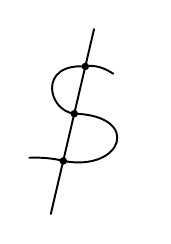
\begin{tikzpicture}[x=0.8cm,y=0.8cm,line width=0.7pt]
\draw (-0.05,0.05) -- (0.64,3);
\draw (0.95,2.28) .. controls (0.8,2.38) and (0.65,2.43) .. (0.5,2.4)
.. controls (-0.25,2.45) and (-0.1,1.7) .. (0.325,1.65)
.. controls (1.4,1.62) and (1.1,0.72) .. (0.15,0.9)
.. controls (0,0.94) and (-0.2,0.96) .. (-0.4,0.95);
\fill (0.5,2.4) circle (0.06);
\fill (0.325,1.65) circle (0.06);
\fill (0.15,0.9) circle (0.06);
\end{tikzpicture}
\end{adjustbox}

([Зачёркнуто: \Unclear{GELFAND-P000837}{multiplicity-cancel}{неразборчивое слово}]
когда есть кратность — выбрасываем)

\underline{И.М.Г.}

\underline{Ф-ла Крофтона:}
длина кривой = среднее число точек, по к-рым её пересекает прямая
(среднее по прямым отн. инвар. меры).

Гриффитс и Чжэнь, вдохновл. раб. Пенроуза, обобщили это на многомерный
[Слева ниже вписано со стрелкой: случай].

\underline{Слой, прох. через точку} $H_0\in U$, \underline{состоит} из
[зачёркнуто: \Unclear{GELFAND-P000837}{slice-cancel-right}{поверхностей}].
[В начале следующей строки зачёркнуто: точек $X$.]
\underline{плоскостей}
\begin{equation*}
\{H\in U\mid \exists i\in\{1,2,\ldots,d\};\ P_i\in H\}.
\end{equation*}
\begin{equation*}
H_0\cdot X=P_1+\ldots+P_d
\end{equation*}
\begin{equation*}
\{H\in U\mid \exists i\in\{1,2,\ldots,d\};\ P_i\in H\}.
\tag{2}
\end{equation*}

Это слоение коразмерности 1
(так \Unclear{GELFAND-P000837}{foliation-note}{зд. плоскости разд. на листы},
сами могут пересечься)

\underline{И.М.Г.}

[Зачёркнуто: \Unclear{GELFAND-P000837}{problem-cancel}{Вопросы}]

\underline{Задача:} есть 3 слоения (трансверс.)
Когда их можно выпрямить?

[Под «есть 3 слоения» вписано:] \underline{на плоск.}

(2 всегда!!)

3 можно выпр. $\Leftrightarrow$ она гексагональна, т. е.

$\approx 1927$ г.

\SourceFigure{GELFAND-P000837}{hexagonal-path}{Рисунок слева: три линии разных направлений пересекаются возле центрального тёмного узла. Вокруг видны малые кружки и утолщённые узлы, соединённые горизонтальными и наклонными отрезками; часть штрихов выделена. На нижнем левом конце диагонали виден стрелочный конец, справа на средней почти горизонтальной линии — большой тёмный стреловидный узел. Точная последовательность обхода и направления отдельных малых стрелок не устанавливаются. Под рисунком и пояснением находятся два отдельных почти горизонтальных отрезка на немного разных уровнях; левый начинается тёмной точкой.}

— такой путь (инфинитезимальный) должен быть
замкнут. — что-то вроде кривизны.

\SourcePage{GELFAND-P000838}{29}

Теперь $m=1$.
\begin{equation*}
X\subset P^n
\end{equation*}
проект. \underline{кривая}

$\check P^n$ — двойств. проект. пр-во.

\begin{equation*}
\check{\mathbb P}^{\,n}\supset U
=\{H\mid H\circ X=d\text{ разных точек}\}.
\tag{3}
\end{equation*}

На $U$ получ. ткань коразмерности 1.

\SourceFigure{GELFAND-P000838}{pencil-diagram}{S-образная кривая проходит через три тёмных центра: верхний справа, средний левее, нижний ещё левее. От каждого центра расходятся многочисленные прямые и слегка изогнутые штрихи, образующие три пучка. Несколько штрихов совпадают или сливаются с кривой и друг с другом; точное количество лучей и все их продолжения не устанавливаются. Подписей не видно.}

\underline{Абелево ур-е для ткани.}

\SourceFigure{GELFAND-P000838}{grid-label}{Слева от формулы (4) небольшой овал, внутри и немного за его краями три изогнутых почти вертикальных штриха и три косых поперечных штриха. Стрелок не видно. Слева над овалом компактная подпись, похожая на $u$ или $U$; её регистр не устанавливается. Геометрия и неуверенная подпись сохранены описанием.}

\begin{equation*}
\begin{cases}
u_1=\mathrm{const}.\\
\vdots\\
u_n=\mathrm{const}
\end{cases}
\tag{4}
\end{equation*}

\underline{Аб. ур-е для ткани имеет вид:}
\begin{equation*}
\sum_{i=1}^{d}f_i(u_i)\,du_i=0,\qquad
\sum_{i=1}^{d}f_i(u_i)\,du_i\in\Omega^1(U).
\tag{5}
\end{equation*}

Между нормальными векторами — зависимость (кокас. векторы),
причём коэффициенты имеют вид $f_i(u_i)$.

\underline{Ранг ткани} $\underset{def}{=}$ макс. число лин. независимых абелевых ур-й,
к-рым она удовлетворяет.

\underline{\underline{Утв. 1}}
\underline{Ранг ткани, построенной по кривой рода $g$, равен $g$.}

[Зачёркнута строка:
\Unclear{GELFAND-P000838}{cancelled-heading}{Еще} теорема 1 —
При условиях
\Unclear{GELFAND-P000838}{cancelled-hypotheses}{$n\ge3,\ d\ge2n$}.]

\underline{Теорема 1} (Chern, 193 ?)
\quad
\underline{Ранг $d$-ткани} $\le\pi(n,d)$.

[Под «Ранг $d$-ткани»:] (в $n$-мерном мн-зии)
\qquad
(число Кастельнуово)

[Слева снизу, со стрелкой к «Ранг $d$-ткани»:] (произв. ткань!)

\begin{equation*}
\pi(n,d)\underset{def}{=}
\text{макс. род кривой степени }d\text{ в }\mathbb P^n,
\qquad \underline{\underline{n,d\ge2}}.
\tag{6}
\end{equation*}

Есть короткая ф-ла
\begin{equation*}
\pi(n,d)=m\left(d-\frac12(m+1)(n-1)-1\right),
\quad\text{где }m=\left[\frac{d-1}{n-1}\right].
\tag{7}
\end{equation*}

\SourcePage{GELFAND-P000839}{unlabelled}
\underline{\underline{Теорема 2.}} (основная)

\underline{Если} $n\geq 3$, $d\geq 2n$ и \underline{$d$-ткань имеет ранг} $\pi(n,d)$,
\underline{то}

1) \underline{Она линеаризуема}

2) \underline{Она продолжается до ткани, получ. из} $X\subset\mathbb{P}^{n}$.

Объясняется связь таких ур-й и абелевых дифференциалов.

\underline{Ссылка.}

\underline{(Sonderdruck aus) Jber. d. Dt. Math.-Verein}, $80$ ($1978$),
13–110

[Под «Sonderdruck aus»: \underline{оттиск} из.]

(\Unclear{GELFAND-P000839}{reference-expansion}{Jahresberichte der Deutschen Math. Vereinigung})

[Ниже зачёркнуто: \Unclear{GELFAND-P000839}{reference-cancelled-word}{неразборчивое слово}.]

Развивается геометрия \underline{проективных связностей}.
[Под «проективных» слева — линия со стрелкой влево.]

\underline{Замолодчиков А.} (Саша)

Пусть есть $S_{ij}^{kl}(\lambda)$

Пусть ещё есть картина:

$L$ прямых, углы $\lambda_1,\ldots,\lambda_L$

$\lambda_i$ в порядке возрастания

(от какой-то прямой

[Слева зачёркнуто: \Unclear{GELFAND-P000839}{cancelled-to}{То}.]

\SourceFigure{GELFAND-P000839}{single-vertex-diagram}{Справа две наклонные прямые пересекаются в обведённой точке. На нижних ветвях видны стрелки от пересечения: вниз влево и вниз вправо. У концов стоят подписи: слева сверху знак, похожий на $l$ или $c$, справа сверху $j$, слева снизу $i$, справа снизу $k$.}

индексы $=1,2,\ldots,N$

\SourceFigure{GELFAND-P000839}{many-lines-diagram}{Ниже и левее рисунка одного узла изображены четыре прямые: почти горизонтальная, восходящая слева направо и две нисходящие с разными наклонами. Видны шесть обведённых попарных пересечений: три на горизонтальной прямой и три выше неё. На концах нескольких прямых короткие косые штрихи, похожие на наконечники стрелок; их направления не во всех случаях различимы. Подписей к этому рисунку нет.}

Узлу — матрица; Хвостам — индексы, по связям — суммирую.

Получ. матрица (большая). Интересно её повед. при $L\to\infty$?

\begin{equation*}
Z^{j_1\ldots j_L}_{i_1\ldots i_L}(\lambda_1,\ldots,\lambda_L).
\end{equation*}

\underline{Проблема 1.} Есть асимптотика

(как \Unclear{GELFAND-P000839}{problem-parenthesis}{сосч. её} — неизвестно)

\begin{equation*}
\ln Z\sim\text{пропорц. числу узлов}\tag{1}
\end{equation*}
[В формуле (1) непосредственно после $Z$ заштрихованы индексы и аргументы:
\Unclear{GELFAND-P000839}{hatched-indices}{$^{j_1\ldots j_L}_{i_1\ldots i_L}(\lambda_1,\ldots,\lambda_L)$}.]

\begin{equation*}
Z\underset{df}{=}Z^{i_1\ldots i_L}_{i_1\ldots i_L}
\qquad\text{(«след»)}\qquad\text{(суммир. по повт.)}\tag{2}
\end{equation*}

Каждой прямой $\leadsto$ параметр $\lambda_j$

(нумеруются лучи по часовой стрелке \underline{$i_1,\ldots,i_L,j_1,\ldots,j_L$})

\begin{equation*}
Z^{j_1\ldots j_L}_{i_1\ldots i_L}
=\sum_{\substack{\text{внутр.}\\\text{отрезкам}}}
\left(\prod_{\substack{\text{точкам}\\\text{пересеч.}}}
S^{**}_{**}(\lambda_a-\lambda_b)\right)\tag{3}
\end{equation*}
[Под знаком суммы между «внутр.» и «отрезкам» зачёркнуто:
\Unclear{GELFAND-P000839}{sum-cancelled-word}{неразборчивое слово}.]

[Приписка под формулой справа:]
естеств. упорядочение из напр. \Unclear{GELFAND-P000839}{ordering-overwritten-ending}{прямых}
[Конец слова переправлен.]

есть горизонт. прямая, к-рую они пересек. в самом низу.

Есть ф-и, к-рые не мен. при паралл. переносе.

\SourcePage{GELFAND-P000840}{30}
\begin{adjustbox}{max width=\linewidth}
\begin{tikzpicture}[x=0.01cm,y=-0.01cm]
\draw (270,185) -- (408,416);
\draw (388,110) -- (349,441);
\draw (202,331) -- (464,124);
\fill (307,248) circle[radius=0.5mm];
\fill (378,192) circle[radius=0.5mm];
\fill (361,337) circle[radius=0.5mm];
\node[left] at (258,169) {$i_1$};
\node[above left] at (384,108) {$i_2$};
\node[above right] at (470,125) {$i_L$};
\node[below left] at (201,347) {$j_L$};
\node[below] at (346,450) {$j_2$};
\node[below right] at (410,423) {$j_1$};
\end{tikzpicture}
\end{adjustbox}

\underline{Ассоциат.} $Z$ не зав. от взаимного распол. прямых.

Достат., чтоб вып. для 3-х прямых:

\SourceFigure{GELFAND-P000840}{three-lines-equality}{Два рисунка трёх попарно пересекающихся прямых, между ними знак равенства. В левом рисунке почти вертикальная прямая проходит слева от пересечения двух диагоналей; в правом — справа. На левом рисунке нижний правый участок нисходящей диагонали сильно утолщён и содержит небольшой светлый промежуток; не вполне ясно, является ли утолщение стрелкой или повторной обводкой. Подписей нет.}

\underline{Утв. 2.} сущ. такие матрицы.

\underline{Об асимптотике.}

\begin{equation*}
\ln Z^{j_1\ldots j_L}_{i_1\ldots i_L}\sim L^2
\qquad\text{при }L\to\infty\tag{4}
\end{equation*}

(\underline{если без ассоциативности}) и асимпт. не зав. от выбора инд. $i$ и $j$.

[Под «асимпт.»: (гл. член.)]

\underline{\underline{Утв. 3.}} Асимптотика при $L\to\infty$

\begin{equation*}
\ln Z(\lambda_1,\ldots,\lambda_L)
=\sum_{a>b=1}^{L}f(\lambda_a-\lambda_b)+\text{остат. член}\tag{5}
\end{equation*}

(своб. эн. большой системы $=$ сумма парных

\underline{\Unclear{GELFAND-P000840}{particle-model-heading}{Мнение}}:
есть $L$ сортов частиц; они движ. по прямым и
сталкиваются; при столкн. они сохр. скорости, но меняют \underline{\underline{цвет}}

[Под «цвет»: (сорт)]

Здесь $Z$ — $S$-матрица;

Есть интерпр., когда $Z$ — стат. сумма

Веса $S$ — $\exp$ от потенциала. (вероятности?)

Есть нач. и \underline{конечные расцветки} $i_1,\ldots,i_L$

\begin{equation*}
j_1,\ldots,j_L.
\end{equation*}

[Горизонтальная разделительная линия.]

\underline{\underline{А. З.}}

\SourceFigure{GELFAND-P000840}{spin-lines-diagram}{Слева небольшой рисунок: почти горизонтальная прямая, почти вертикальная изогнутая линия и две диагонали. Восходящая диагональ проходит от нижнего левого конца к верхней части почти вертикальной линии; нисходящая идёт сверху слева вниз вправо. Пересечения около горизонтальной и почти вертикальной линий густо обведены и сливаются, поэтому число отдельных узлов здесь не вполне различимо. Подписей к линиям нет.}

\underline{спиновые}
\newline
\underline{переменные} — в многоугольниках; взаимод. ближ. соседей;

$S$ \Unclear{GELFAND-P000840}{s-expression-note}{не с… выражается}.

\begin{equation*}
Z=\sum_{\{\sigma\}}e^{-\beta H}
\qquad
H=\sum h(\sigma_A,\sigma_B)
\end{equation*}

Точно счит. стат. суммы — все такие!

\underline{Для модели Изинга:}

\begin{equation*}
S_{ij}^{kl}=\frac{ijkl+1}{2}e^{-\frac{\beta}{2}(i+j+k+l)}
\end{equation*}

(после перехода к дуальной решётке)
\SourcePage{GELFAND-P000841}{unlabelled}
% Original inspected at 2408 x 3448 pixels. Review coordinates use (left, top, right, bottom), origin at upper left.
% Full text review at 3x: (60,0,2260,625); (150,615,2340,1180); (150,1150,2340,1680); (160,1670,2260,2170); (70,2150,2350,2860); (40,2820,2320,3448).
% Further close reviews: header (135,120,1320,225) 4x; meeting (170,245,1760,340) 4x; names (185,320,1765,400) 4x; Hawking note (855,475,1370,625) 5x.
\underline{24.9.79 г.}\qquad \underline{Сем. Гельфанда}

\underline{Рената Эрнестовна КАЛЛОШ} о \underline{конфер. в Кембридже}

(физик)

(месячное раб. совещ. по кв. гравитации, прим. 40 чел.)

20 чел. из USA; в т. числе \underline{Chern, Singer, Milnor, Penrose};

Hawking, De Witt, Sciama, Coleman, Jackiw

[Под именем Hawking, с короткой вертикальной чертой:] претендент на св. кресло Ньютона

% Gibbons and topology: (290,602,1780,700) 4x; abbreviation (1180,602,1460,700) 8x; (140,705,2330,915) 4x.
\underline{Gibbons} — физик, раб. с Хокингом — \Unclear{GELFAND-P000841}{gibbons-abbreviation}{докл.? / сем.?} о кв. гравитации

\underline{Идея}: надо принять во внимание эффекты нетрив. топологии пр-ва/времени в малом.

(много маленьких „ручек“).

Теория не построена, но есть значит. продвижения.

В \Unclear{GELFAND-P000841}{hawking-coauth-abbreviation}{соавтст.?} \underline{Hawking}:

1) \underline{Space-time foam} (пена) — вышло в \underline{Nuclear Physics}

(обычн. журн.)

% Nuclear Physics note: (1580,950,2330,1110) 5x. Page/Atiyah sentence: (835,1115,1740,1235) 5x.
2) \underline{Page, Atiyah} — что-то в поле \Unclear{GELFAND-P000841}{page-atiyah-abbreviation}{изл.? / изв.?} гравитонов

(из гр. Hawking)

% Coleman text: (900,1280,1800,1450) 5x; instanton sentence (560,1410,1550,1535) 5x and (900,1420,1380,1520) 6x.
3) \underline{Coleman, Jackiw} — о гравит. с учётом топ. чисел.

о Янге-Миллсе.

(есть обзор о методах инстантонов)

% Milnor and following line: (200,1540,1630,1740) 4x. Singer: (217,1780,1240,1865) 4x.
4) \underline{Милнор} — классиф. 4-мерных мн-зий

Кто-то о рассл. на 4-мн-зиях.

5) \underline{Зингер} — о сигнатуре 4-мн-зия.

\underline{О супермногообразиях}

Счит. путём к квантованию

De Witt пишет книгу о супермн-зиях

Singer чит. лекции — „ —

\begin{center}
— $\cdot$ —
\end{center}

% Result heading: (305,2295,2200,2405) 4x. Author note: (1615,2385,2365,2550) 4x; cancelled name (1625,2390,1855,2468) 10x.
\underline{Нечто, что независ. получ. докладчицей и кем-то из участников конф.}

[Справа:] [Зачёркнуто: \Unclear{GELFAND-P000841}{cancelled-author}{Christen?}] Christensen, Duff;

\underline{Kallosh} — докладчица

Рассм. ур-е
\begin{equation*}
\Delta[A,B]\,\Phi[A,B]=0 \tag{1}
\end{equation*}

Здесь
% Spinor definition (330,2580,1500,2820) 5x; group note (1400,2610,2240,2775) 5x; phi forms (340,2588,418,2675) and (720,2420,800,2515) 10x.
\begin{equation*}
\phi[A,B]=\Psi_{\alpha_1\ldots\alpha_{2A};\dot\alpha_1,\ldots,\dot\alpha_{2B}}(x)
\end{equation*}
— мультиспинор, преобр. по группе $SO(4)$

$x\in$ [Зачёркнуто: \Unclear{GELFAND-P000841}{cancelled-space-symbol}{нечитаемый знак}] $R^4$.

% Operator note: (340,2835,2240,2975) 4x. Equation (2): (425,3040,2010,3190) 5x; separator (578,3080,660,3170) 10x.
$\Delta$ — какой-то оператор; что-то от Ходжа-де Рама

здесь есть и пол. Дирака

\begin{equation*}
S=A+B,\qquad T=A-B.
\end{equation*}

\begin{equation*}
n[S;T]-n[s;T-1]=4^{s-1}\left[\left(T-\frac12\right)\chi+\left(s-\frac13\right)\frac12p\right]. \tag{2}
\end{equation*}
\Unclear{GELFAND-P000841}{formula-two-s-case}{В (2) регистр $S/s$ различается неуверенно.}

% Definition of n: (520,3200,1550,3380) 4x, (560,3210,910,3300) 6x; characteristic numbers (1570,3220,2270,3420) 4x.
[Под $n$, с короткой вертикальной чертой:] число 0-х мод

(разм. пр-ва реш., с спином $A$ и $B$);

$\chi,p$ — числа Эйлера, Понтрягина

\SourcePage{GELFAND-P000842}{66}
% Original inspected at 2408 x 3448 pixels. Review coordinates use (left, top, right, bottom), origin at upper left.
% Full text review at 3x: (45,0,2335,620); (120,590,2240,1250); (120,1240,2340,1880); (120,1820,2320,2020); (145,2020,2310,2410); (140,2400,2140,2630); (135,2610,2340,3040); (90,3010,2380,3448).
Здесь есть теоремы Гаусс-Боне, Атья-Зингера, и т. п.

% Equation (3) overtraced sign: (645,135,845,260) 10x.
\begin{equation*}
n[A,B]-2n\left[A\overset{?}{-}\frac12,B\right]=4^{A+B-1}\left(A-\frac7{12}\right)\left(\chi+\frac12p\right). \tag{3}
\end{equation*}
\Unclear{GELFAND-P000842}{formula-three-sign}{Между $A$ и $1/2$ густо затушёванный знак; минус дан лишь как возможное чтение.}

О ненулевых модах:

% Equation (4): (240,355,1230,500) 5x; separator (365,390,455,470) 10x.
\begin{equation*}
m[S;T]=m[S]=4^s m[0] \tag{4}
\end{equation*}
\Unclear{GELFAND-P000842}{formula-four-s-case}{В показателе степени (4) $s$ или $S$.}

[Под $m[S;T]$:] ненулевые моды.

\begin{equation*}
\Delta\Psi_i=\lambda_i\Psi_i \tag{5}
\end{equation*}

В супергравитации ненулевые моды сокращ. и ост. вклад лишь нулевых.

% Self-duality line: (220,727,1320,835) 5x.
(3) [Зачёркнуто: \Incomplete{GELFAND-P000842}{selfduality-cancellation}{Слово под густым зачёркиванием не прочитано.}] лишь если мн-зие \underline{самодуально}.

Раньше что-то док. Хокинг.

Коэфф. в \Unclear{GELFAND-P000842}{heat-abbreviation}{теплопров.?}

\begin{equation*}
B_4=n+m
\end{equation*}

Доказали, что функц. интеграл не имеет \underline{расходимостей}.

(в гравитации)

% Dokladchitsa line: (210,1210,1330,1300) 4x.
Докладчица — тоже что-то сделала.

Интересная зад.: то же на супермногообразии.

Зингер сейчас этим занимается.

Возникла группа $SO(8)$, что-то было не так.

% French-group cancellation: (740,1630,1100,1725) 8x.
Франц. группа: [Зачёркнуто: \Incomplete{GELFAND-P000842}{french-group-cancellation}{Группа букв и знаков не прочитана полностью; в конце различимо (8).}] симметрия $E_7$ и

\begin{equation*}
\underline{E_7\longrightarrow SU(8)}
\end{equation*}

тогда \underline{расш. супергравитация}

\begin{equation*}
\dim E_7=133
\end{equation*}

($E_7$ — искл. группа Ли)

\underline{Интересно}

% Overwritten mark before sdelat: (254,1900,360,2000) 10x.
[Зачёркнуто: \Unclear{GELFAND-P000842}{index-theorem-cancelled-mark}{нечитаемый знак}] \underline{сделать супертеорему об индексе}

\underline{Замечания:}

% F4 insertion/cancellation: (505,2113,645,2230) 10x; Jordan wording (1370,2130,2300,2230) 5x, final abbreviation (2010,2150,2265,2225) 8x, ending (1830,2125,2270,2250) 7x.
$F_4$

[Вставлено над строкой:] Эрмитовы

[Зачёркнуто: \Incomplete{GELFAND-P000842}{f4-cancellation}{Зачёркнутое начало строки перед словом «матрицы» не прочитано.}] \underline{матрицы 3-го пор. из октав}; в них строится \Unclear{GELFAND-P000842}{jordan-abbreviation}{йорданова сист.? / йорданово слож.?}

произведение $\frac12(AB+BA)$.

% Word algebry checked at (1730,2320,2070,2430), 8x.
надо взять группу автоморфизмов этой йорд. алгебры; получим $F_4$

\underline{Черн} — советник кит. президента — раб. в \underline{Чикаго}.

\underline{Янг} чит. лекции в Китае перед тысячной ауд.

% Einstein lines: (220,2725,1470,2820) 4x; (1470,2790,2340,2900) 5x; (225,2880,2340,3055) 4x; quote end (1785,2890,2350,3050) 8x.
\underline{И. М. Г.} — \underline{что физики говорили} об Эйнштейне.

а) Э. и Н. Бор — самые крупные физ. в столетии

б) Э. в молодости сделал прекр. раб., но потом 30–40 лет заним. ерундой (пыт. созд. единую теорию поля).

в) \underline{Э.: Борну}: „Хочу пригл. тебя в Принстон, но с такой старой клячей, [вставлено над строкой: как я,] здесь всерьёз никто не считается“.

% Left margin note: (128,2960,305,3060) 8x.
[На левом поле:] \underline{Доска.}

% Bottom figures and associated text: (90,3010,2380,3448) 3x; text and right hatching (1005,3070,1800,3350) 4x.
\SourceFigure{GELFAND-P000842}{leaf-branch-diagram}{Слева внизу два вытянутых листообразных контура, расходящихся от общей нижней точки влево и вправо вверх. Внутри каждого проходит ветвящийся стержень с короткими боковыми отростками; под общей точкой маленький прямоугольный штрих. Точные соединения и смысл линий оставлены для проверки по оригиналу.}

\underline{связь теор. физики с математикой:}

в фунд. вещах

(рисунок Янга)

\SourceFigure{GELFAND-P000842}{lower-right-hatching}{Справа от слов «в фунд. вещах» и «рисунок Янга» две почти вертикальные линии и густая группа наклонных штрихов, образующая вытянутую клиновидную фигуру. Отдельных читаемых подписей не видно; точная структура штрихов и их связь с левым рисунком не установлены.}

% Original frames inspected directly at 2408 x 3448 pixels.
% Coordinates below are (left,top,right,bottom) in original pixels.
\SourcePage{GELFAND-P000843}{unlabelled}
% Full-frame inspection included every margin; no confident leaf label was visible.
% General 3x crops: (180,110,1400,950); (1420,40,2200,375);
% (330,940,2300,1530); (320,1500,2360,1740); (200,1630,1430,1960);
% (200,1940,2240,2460); (290,2450,1610,2710); (80,2700,1900,3448).
\underline{В. Е. Захаров.}

% Upper-right marginal note, (1420,40,2200,375), inspected 3x.
[На поле справа; запись объединена левой квадратной скобкой:]

\underline{об ОТО читать:}

Дирак; \quad Ландау, Лифшиц;

Вайнберг;

Хокинг, Эллис;

[Основная запись:]

Математич. задача: [Подчёркнуто волнистой линией.]

\begin{equation*}
k=(k_1,\ldots,k_N)
\end{equation*}

Рассм. ф-ю $\omega(k)$ (вещественную) и пр-во пар
$(k_1,k_2)$ размерности $2N$ и
\Unclear{GELFAND-P000843}{intro-short-word}{так}
ур-е
% intro-short-word: (1190,590,1460,700), inspected 5x.

\begin{equation*}
(1)\qquad \omega(k_1+k_2)=\omega(k_1)+\omega(k_2)
\end{equation*}

% Hypersurface line: (360,820,1730,933), inspected 3x.
% Lower-case n in the exponent is retained from the source.
$\omega$ — нелин. $\Rightarrow$ получ. поверхность $\Gamma$ в $R^{2n}$

Сущ. ли другая ф-я $f$, удовл. тому же ур-ю на $\Gamma$:
\begin{equation*}
f(k_1+k_2)=f(k_1)+f(k_2)
\end{equation*}
и не отлич. от $\omega$ на линейную?
% This line inspected at (365,1140,1450,1250), 3x.

% cancel-before-situation: (355,1240,510,1335), inspected 8x.
[Зачёркнуто: \Unclear{GELFAND-P000843}{cancel-before-situation}{Это}]
Эта сит. исключительна, т.к. размерность большая

% Idea line: (360,1350,2335,1500), with ending (1540,1340,2340,1460), 3x.
Идея Зах. и Шульмана: как получать все ур-я, имеющие беск. число 1-х
интегралов.

\underline{Пример:} \quad \underline{$N=2$.}

Задавать будем с пом. параметризации, $\vec{k}=(p,q);$

% Small interline note: (342,1587,1005,1668), inspected 4x.
[Мелкая приписка под началом строки:]
2 независим \Unclear{GELFAND-P000843}{example-small-word}{вел-х}
$\omega$ зад. так:

$\omega(p,q),$
\begin{equation*}
(2)\qquad
\left[
\begin{aligned}
p&=\xi_1-\xi_2\\
q&=a(\xi_1)-a(\xi_2)\\
\omega&=b(\xi_1)-b(\xi_2)
\end{aligned}
\right.
\end{equation*}

Другая
\Incomplete{GELFAND-P000843}{cancelled-other-function}{Между словами «Другая» и «ф-я» зачёркнута короткая запись; её текст не читается.}
ф-я $f$:
% cancelled-other-function: (597,1954,704,2037), inspected 10x.

\begin{equation*}
(3)\qquad
\left[
\begin{aligned}
p&=\xi_1-\xi_2\\
q&=a(\xi_1)-a(\xi_2)\\
f&=c(\xi_1)-c(\xi_2)
\end{aligned}
\right.
\qquad c\text{ — другая ф-я (любая)}
\end{equation*}
\Unclear{GELFAND-P000843}{third-system-rewritten}{В третьей строке предварительно прочитано $f=c(\xi_1)-c(\xi_2)$; левая буква похожа также на $\varphi$, первая буква справа — на $e$.}
% third-system-rewritten: (530,2280,1120,2410), inspected 5x.
% The description to its right: (1430,2300,2220,2410), inspected 3x.

Вопрос: явл. ли это общей конструкцией?

Идея: параметризацию $\Gamma$ зададим (оно 3-мерно)
% The source's literal "оно 3-мерно" inspected at (1240,2590,1700,2695), 4x.
\begin{equation*}
(4)\qquad
\left\{
\begin{aligned}
p_1&=\xi_1-\xi_2\\
q_1&=a(\xi_1)-a(\xi_2)\\
p_2&=\xi_2-\xi_3\\
q_2&=a(\xi_2)-a(\xi_3)
\end{aligned}
\right.
\end{equation*}

\begin{equation*}
\underbrace{p_1+p_2}_{p_3}\qquad
\underbrace{q_1+q_2}_{q_3}\qquad
p_3=\xi_1-\xi_3
\end{equation*}

\Unclear{GELFAND-P000843}{bottom-connector}{и} т.д.
% bottom-connector: (440,3348,635,3438), inspected 6x.

\SourcePage{GELFAND-P000844}{67}
% Full-frame inspection included the upper-right handwritten label 67.
% General 3x crops: (100,30,1820,470); (160,470,1170,880);
% (200,840,2260,1060); (220,1050,1160,1550); (1410,1250,2280,1640);
% (280,1590,1750,2070); (260,2040,1100,2680); (380,2690,2150,2890);
% (200,2890,2180,3390).
\Incomplete{GELFAND-P000844}{top-cancelled}{Над первой строкой зачёркнута короткая запись; её текст не читается.}
% top-cancelled: (248,55,392,146), inspected 8x.

Отсюда или вырождена, то серьезно (функц. параметр).
% The source's literal connector and next word were checked separately:
% (383,140,538,202), 6x; (942,142,1153,212), 4x. Syntax is not supplied.

Сущ. метод констр. систем с предст. Лакса (Захаров-Шабат)
% "предст." inspected at (976,228,1171,301), 4x.

\begin{equation*}
(5)\qquad \frac{\partial L}{\partial t}-\frac{\partial A}{\partial y}+[L,A]=0
\end{equation*}

\begin{align*}
L&=\frac{\partial^n}{\partial x^n}+\ldots\\
A&=\frac{\partial^m}{\partial x^m}+\ldots
\end{align*}

(5) — нелин. сист. ур-й на коэфф.

Рассм. ее \underline{линеаризацию.}
[Под строкой, с соединяющей чертой: (отбросим нелин. члены)]
Это сист. с пост. коэфф., она реш. методом Фурье.

\begin{equation*}
u_j\sim\exp(-\omega t+qy+px)
\end{equation*}
\begin{equation*}
\omega=\omega(p,q)
\end{equation*}

\Unclear{GELFAND-P000844}{systems-phrase-start}{Те} сист. выглядят так как в
% systems-phrase-start: (220,1230,470,1305), inspected within the 3x middle crop.
% Last isolated "в" checked at (1001,1240,1070,1307), 10x; the clause stops here.

$a(\xi)$ — символ опер. $L$

$b(\xi)$ — ″ — $A$

[На поле справа, отделено двумя вертикальными чертами:]
\begin{align*}
L&=L_0+\delta L\\
A&=A_0+\delta A
\end{align*}
$\delta L,\delta A$ — всё, что содержит переменные коэфф.

[Основная запись:]

Вырожд. законы дисп. связаны с обр. задачей.
% This phrase checked at (285,1580,1555,1690), 4x.

\begin{align*}
p&=\xi_1-\xi_2\\
q&=\ell(\xi_1)-\ell(\xi_2)\\
\omega&=a(\xi_1)-a(\xi_2)
\end{align*}
$a,\ell$ — симв. $A_0,L_0$.
% The change from a,b above to ell,a here is retained literally.

Рассм. ур-е Г.-Л.-М.:
\begin{equation*}
F+K+K\oplus F=0
\end{equation*}
% The circled plus is directly visible: (819,2188,876,2260), inspected 10x.
\begin{align*}
\frac{\partial F}{\partial t}+[L_0,F]&=0\\
\frac{\partial F}{\partial y}+[A_0,F]&=0
\end{align*}
% The heavily retraced plus on the second line was inspected
% at (574,2450,644,2540), 10x; the visible final sign is retained.
\begin{equation*}
K=-F
\end{equation*}

\begin{equation*}
F=\exp\bigl(\xi_1x-\xi_2z+[\ell(\xi_1)-\ell(\xi_2)]y+[a(\xi_1)-a(\xi_2)]t\bigr)
\end{equation*}
\Unclear{GELFAND-P000844}{exponential-overwritten-coordinate}{Буква после $\xi_2$ предварительно прочитана как $z$; она густо переписана.}
% exponential-overwritten-coordinate: (928,2735,1007,2833), inspected 10x.
% All displayed signs and the source's order of ell,a,L_0,A_0 are retained.

Здесь связь уст., когда $\ell$ и $a$ — полиномы; можно уст. связь для
рац. функций.
% The retraced ell here checked at (967,2890,1059,2980), 8x.

\begin{equation*}
\ell=\xi^2,\qquad a=\xi^3
\end{equation*}
[Под двумя равенствами проведена общая нижняя скобка.]

$L,A$ ищутся — получ. KdV.
% Final caption checked at (335,3180,1360,3330), 3x.

\SourcePage{GELFAND-P000845}{unlabelled}
% Оригинал 2408 x 3448; координаты (left,top,right,bottom), начало в левом верхнем углу.
% Полный оригинал просмотрен непосредственно; все текстовые области проверены при x3, детали при x4--x10.
% top (50,70,2250,430), x3; margin-left (45,290,265,390), x8.
Интегр. обр. задачи $\Rightarrow$ закон дисп. вырожден.

\begin{center}— · —\end{center}

Матрицы $L$ и $A$: уже не обязательно

\underline{Альтерн.}\quad Если ур-е интегр., а закон дисп. невыр., то
взаимод. $\equiv 0$ на
\Unclear{GELFAND-P000845}{resonance-abbreviation}{рез-… [окончание сокращения неясно]}.

\begin{center}— · —\end{center}

% dispersion (392,433,1735,590), x4. Правая скобка перед вторым равенством не добавлена.
\begin{equation*}
\omega=\frac18\bigl[(p+\frac qp)^3-(-p+\frac qp)^3
=\frac14\bigl[p^3+\frac{3q^2}{p}\bigr]
\end{equation*}
\Unclear{GELFAND-P000845}{dispersion-bracket}{[Перед вторым равенством закрывающая квадратная скобка не видна.]}

% kp (250,430,1800,1130), x3; kp-relation (600,690,688,805), x10.
\underline{Ур-е Кад.-Петв.:}
\begin{equation*}
u_t\;\text{[исправленный знак]}\;\frac14
\left(u_{xxx}+6uu_x-3\int_{-\infty}^{x}u_{yy}\,dx\right)
\end{equation*}
\Unclear{GELFAND-P000845}{kp-relation}{$=$ / $+$ [знак переписан поверх других штрихов].}

% kp-note (470,835,1250,932), x6; kp-lower-text (270,930,2140,1130), x3.
выше \Unclear{GELFAND-P000845}{kp-note}{выписал / выписан} её символ.

$\xi^2$ и $\xi^3$ одеваем — получ. К.-П.-ур-е.

Т.е. К.-П. обладает именно этим зак. дисп. (как в примере)

\begin{center}— · —\end{center}

% pair (170,1140,1730,1670), x3; heading-action (685,1130,1110,1240), x6.
\underline{Эксперим. факт.:} одеваем пару
\begin{equation*}
L_0=\begin{pmatrix}1&0\\0&-1\end{pmatrix}\frac{\partial}{\partial x},
\qquad
A_0=\begin{pmatrix}1&0\\0&1\end{pmatrix}\frac{\partial^2}{\partial x^2}
\end{equation*}
Получим
\begin{equation*}
L=\begin{pmatrix}1&0\\0&-1\end{pmatrix}\frac{\partial}{\partial x}
+\begin{pmatrix}0&\psi\\\bar\psi&0\end{pmatrix}
\end{equation*}
% Нижний левый элемент (1350,1480,1475,1630), x8: bar(psi), без минуса.
и ур-е
% system (80,1660,2150,2330), x3; name-ds (390,2080,1260,2215), x4.
\begin{equation*}
\text{(6)}\quad
\left\{\begin{aligned}
i\frac{\partial\psi}{\partial t}-\frac{\partial^2\psi}{\partial x^2}
+\frac{\partial^2\psi}{\partial y^2}+u\psi&=0\\
\left(\frac{\partial^2}{\partial x^2}+\frac{\partial^2}{\partial y^2}\right)u
&=\left(\frac{\partial^2}{\partial x^2}-\frac{\partial^2}{\partial y^2}\right)|\psi|^2
\end{aligned}\right.
\end{equation*}
сист. Д… — Стюартсона (см. гидродин., теор. пов. волн)

Возьмём преобр. Фурье. Получим сист. вида:
% fourier (320,2330,2408,2850), x3; fourier-symbol (575,2340,720,2480), x8.
\begin{gather*}
\psi\to a(k)\\
i\frac{\partial a(k)}{\partial t}=\frac{\delta H}{\delta a(k)}
\end{gather*}
% Над a(k) в знаменателе вариационной производной черта не добавлена: в оригинале её не видно.
\Unclear{GELFAND-P000845}{variational-denominator}{[В знаменателе записано $\delta a(k)$ без черты; возможная особенность обозначений или ошибка источника.]}
\begin{equation*}
\begin{aligned}
H={}&\int\omega_k|a_k|^2\,dk\\
&+\int\text{[неясный коэффициент]}_{kk_1k_2k_3}
\bar a_k\bar a_{k_1}a_{k_2}a_{k_3}
\delta_{k+k_1-k_2-k_3}\;\text{[неясная мера]}
\end{aligned}
\end{equation*}
\Unclear{GELFAND-P000845}{hamiltonian-coefficient}{$w$ / $W$; верхний правый штрих может принадлежать букве либо отдельному знаку.}
\Unclear{GELFAND-P000845}{hamiltonian-measure}{$dk_1\,dk_3$ / $dk_2\,dk_3$; первый индекс и переписанные штрихи неясны.}

% bottom (500,2900,2240,3200), x4. Во втором знаменателе сохранены видимые плюсы, не заменены минусами.
\begin{equation*}
w=\frac{(p_1-p_3)^2-(q_1-q_3)^2}{(p_1-p_3)^2+(q_1-q_3)^2}
+\frac{(p_2-p_4)^2-(q_2-q_4)^2}{(p_2+p_4)^2+(q_2+q_4)^2}
\end{equation*}
\Unclear{GELFAND-P000845}{bottom-denominator-signs}{[Во втором знаменателе видны $p_2+p_4$ и $q_2+q_4$; асимметрия с числителем может быть ошибкой источника. Плюсы сохранены.]}

\SourcePage{GELFAND-P000846}{68}
% Оригинал 2408 x 3448; координаты (left,top,right,bottom), начало в левом верхнем углу.
% Полный оригинал просмотрен непосредственно; все текстовые области проверены при x3; детали x4--x8.
% page-label (2220,60,2395,175), x4: 68. top (150,30,1180,625), x3.
В пр-ве $k_1,k_2,k_3,k_4$

рассм. ур-е
\begin{gather*}
\omega(k_1)+\omega(k_2)=\omega(k_3)+\omega(k_4);\\
k_1+k_2=k_3+k_4
\end{gather*}
\Incomplete{GELFAND-P000846}{cancelled-top-line}{Строка под равенствами густо зачёркнута; слова под штриховкой не прочитаны.}

Оказ., что $w|_\Gamma=0$.

% upper (180,625,2390,915), x3; reference (1180,800,1780,900), x5.
\underline{Гип. Арнольда:}
Это — теор. Пуанкаре об интегрируемости. (когда есть 1-й инт., незав. от эн.)

Усл. Пуанкаре: ампл. рез. гармоник должны быть 0

(см. Пуанкаре, Неб. мех., или Арнольд: доп. главы)

% poincare (230,920,2110,1550), x3; angle-symbol (735,1025,925,1148), x8.
\underline{Пуанкаре:} гамильтониан
\begin{equation*}
H=H_0(p)+\varepsilon\sum h_k(p)e^{ikq}
\end{equation*}
$p=I$, $q=$ \Unclear{GELFAND-P000846}{angle-symbol}{$\varphi$ / $\psi$}.

Когда $\exists$ инт. $F(p,q,\varepsilon)$ (по $q$ всё периодично),

[Под $F$:] незав. от $H$.

\underline{Необх. условие:} составим $\lambda=\frac{\partial H_0}{\partial p}$
и наложим на неё усл. невыр.

$\det\left|\frac{\partial\lambda}{\partial p}\right|\ne0$ — одно из усл. невыр. (всего их 2)

% condition (225,1530,1910,2115), x3; harmonic-condition (490,1810,1350,1960), x5.
Интегралов нет, если
\begin{equation*}
\Gamma:\quad\langle k,\lambda(p)\rangle=0
\end{equation*}
Усл. Пуанкаре:
\begin{equation*}
\underline{h_k|_{\Gamma_k}=0},\qquad k\in\mathbb Z^n.
\end{equation*}
если оно наруш. беск. число раз, то интеграла нет

Идея. $\lambda\leftrightarrow\omega$.

% curves (170,2140,2070,2770), x3; diagram-01 (385,2270,565,2580), x8.
\underline{Арн.}\quad ф-лы (2) означают, что есть \underline{пов. переноса.}

\SourceFigure{GELFAND-P000846}{diagram-01}{Слева от текста две кривые сходятся возле небольшой петли: одна идёт снизу слева вверх направо, другая от области петли изгибается вниз направо и далее почти вертикально вниз. Подписей не видно; утолщения у левого конца и возле петли не позволяют уверенно установить наличие и направление стрелок.}

двигаем 2-ю кривую по 1-й,

параллельно перенося её

\underline{Кривые:}
\begin{equation*}
\begin{aligned}
p&=\xi_1;&\qquad p&=-\xi_2\\
q&=a(\xi_1);&q&=-a(\xi_2)\\
\omega&=b(\xi_1);&\omega&=-b(\xi_2),
\end{aligned}
\end{equation*}
% curve-motion (345,2690,1215,2790), x5.
Кривая двиг. сама по себе.

% bottom (145,2780,2400,3310), x3; final-text (255,3000,2408,3330), x4.
\underline{Захаров.}
\begin{equation*}
\omega_1(k_1+k_2)=\omega_2(k_1)+\omega_3(k_2)
\end{equation*}
получ. общие пов. переноса.

\begin{center}— · —\end{center}

\underline{Рецепт действий.}\quad Проверяем, вырожд. ли закон дисп.; затем смотрим

0 или не 0 — там гам. взаимод.

Что если интегралы начин. сразу с высших порядков?

\SourcePage{GELFAND-P000847}{unlabelled}
% Оригинал 2408 x 3448. Координаты ниже: (left,top,right,bottom), начало в левом верхнем углу.
% Полный оригинал просмотрен; текстовые кропы увеличены в 3 раза; детали зачёркиваний — до 10 раз.
% top-heading (90,70,1090,305), x3; top-formula (330,310,1130,500), x3.
\underline{\underline{Арн.}}\quad \underline{биркгоф.}
[«биркгоф.» подчёркнуто волнистой линией.]
\begin{equation*}
H=\sum\omega_k z_k\bar z_k+\ldots
\end{equation*}
[Перед следующей суммой зачёркнуто:
\Unclear{GELFAND-P000847}{cancelled-h}{$H=$ / $H$}.]
\begin{equation*}
\sum\omega_k(p_k^2+q_k^2)+\ldots
\end{equation*}
% top-right-formula (1300,310,1730,560), x3.
[Справа:]
\begin{gather*}
z=p+iq\\
\Pi_k=z_k\bar z_k
\end{gather*}
% birkhoff-text (320,510,1480,720), x3; formal-series (1680,505,2390,690), x3.
биркгоф: \underline{в нерез. случае прив. к $H(\Pi_k)$.}

(если $\omega_k$ независимы)

[Справа:] (на уровне форм. рядов)

% reading-list-start (140,700,1780,1025), x3.
\underline{И. М. Г.}\quad \underline{Краткий список того, что надо знать.}

1. \underline{Соврем. абстр. язык}\quad
(см. напр., 1-ю часть кн. \underline{Кириллова})

% Аннотация под пунктом 1: (1060,850,1820,1015); показаны ступенчатая линия и стрелка вниз.
[Под строкой:]
\begin{center}
\begin{adjustbox}{max width=\linewidth}
\begin{tikzpicture}[x=1cm,y=1cm]
\draw (0,1.05)--(2,1.05)--(2,0)--(6,0);
\draw[->] (3,1.2)--(3,0.72);
\node at (3,0.35) {\underline{словарь}};
\end{tikzpicture}
\end{adjustbox}
\end{center}

% reading-list-second (200,930,1430,1140), x3.
2. \underline{Арнольд}: дифф. ур. + доп. главы

(чтобы привыкнуть к анализу)

% reading-list-third (210,1090,2370,1385), x3; algebra-cancelled (1160,1110,2040,1220), x4.
3. \underline{По алгебре}: 2 главы кн. \underline{Серра} по
[зачёркнуто: \Unclear{GELFAND-P000847}{algebra-cancelled}{представлениям?}]
предст. кон. групп.

[Над началом следующей строки зачёркнуто: все.]

все кроме \underline{1 гл.} кн. \underline{Серра} по гр. и алг. Ли
(особенно, посл. главу)

% reading-list-linear (300,1370,1330,1530), x3; linear-cancelled (575,1368,735,1425), x10.
\Incomplete{GELFAND-P000847}{linear-cancelled}{Небольшое зачёркнутое слово над строкой «Лин. алгебра» не прочитано.}

\underline{Лин. алгебра}: Гельфанд; Мальцев

% reading-list-geometry (210,1500,2310,1760), x3; geometry-otn (1910,1490,2330,1645), x5.
4. \underline{Дифф. геометрию} в 2-х вар.: старый тензорный
(см. \underline{Дирак} о теории отн.; и \underline{Ландау и Лифшиц})

совр. вар.: векторные рассл. и связности.

% reading-list-representations (215,1750,1450,2010), x3.
5. \underline{Представления}: Г. Вейль

лекции Рака\quad Racah.

Гельфанд, Минлос, Шапиро

\end{document}
